% =====================================================================
% Evidence Debt: Measuring the Accumulated Cost of Missing Operational
% Evidence in Cloud-Native Systems
%
% Journal-length manuscript, IEEE-Transactions-style formatting on the
% base article class (content transplants directly into IEEEtran /
% llncs / elsarticle for submission).
% =====================================================================
\documentclass[10pt,twocolumn]{article}
\PassOptionsToPackage{hyphens}{url}

% ------------------------- fonts and layout --------------------------
\usepackage[T1]{fontenc}
\usepackage[utf8]{inputenc}
\usepackage{mathptmx}
\usepackage[scaled=0.90]{helvet}
\usepackage{courier}
\usepackage[letterpaper,left=0.66in,right=0.66in,top=0.73in,bottom=0.95in]{geometry}
\setlength{\columnsep}{0.25in}
\usepackage{microtype}

% ------------------------- packages ----------------------------------
\usepackage{amsmath,amssymb,amsthm}
\usepackage{graphicx}
\usepackage{xcolor}
\usepackage{booktabs}
\usepackage{multirow}
\usepackage{threeparttable}
\usepackage{enumitem}
\usepackage{listings}
\usepackage{caption}
\usepackage{titlesec}
\usepackage{tikz}
\usetikzlibrary{arrows.meta,positioning,calc,shapes.geometric,fit,backgrounds,decorations.pathreplacing,matrix}
\usepackage{pgfplots}
\usepgfplotslibrary{groupplots}
\pgfplotsset{compat=1.17}
\definecolor{serA}{RGB}{0,84,147}     % deep blue
\definecolor{serB}{RGB}{202,108,2}    % orange
\definecolor{serC}{RGB}{0,122,83}     % green
\definecolor{serD}{RGB}{150,30,90}    % magenta
\pgfplotsset{
  edplot/.style={
    width=0.52\textwidth, height=4.35cm,
    tick label style={font=\fontsize{7}{8}\selectfont},
    label style={font=\fontsize{7.4}{8.4}\selectfont},
    title style={font=\fontsize{7.6}{8.6}\selectfont},
    legend style={font=\fontsize{6.6}{7.6}\selectfont, draw=black!40,
                  fill=white, fill opacity=0.9, text opacity=1},
    grid=major, grid style={black!12},
    xlabel={degradation level $p$ (\%)},
  }
}
\usepackage{balance}
\usepackage[hidelinks]{hyperref}
\usepackage{url}
\usepackage[capitalize,noabbrev]{cleveref}

% ------------------------- IEEE-style sectioning ---------------------
\renewcommand{\thesection}{\Roman{section}}
\renewcommand{\thesubsection}{\thesection-\Alph{subsection}}
\renewcommand{\thesubsubsection}{\thesubsection.\arabic{subsubsection}}
\titleformat{\section}{\centering\normalsize\scshape}{\thesection.}{0.5em}{}
\titleformat{\subsection}{\normalsize\itshape}{\Alph{subsection}.}{0.5em}{}
\titleformat{\subsubsection}{\normalsize\itshape}{\arabic{subsubsection})}{0.5em}{}
\titlespacing*{\section}{0pt}{2.2ex plus .6ex minus .2ex}{1.2ex plus .3ex}
\titlespacing*{\subsection}{0pt}{1.8ex plus .5ex minus .2ex}{0.8ex plus .2ex}
\titlespacing*{\subsubsection}{0pt}{1.4ex plus .4ex minus .2ex}{0.6ex plus .2ex}

% ------------------------- captions ----------------------------------
\captionsetup[figure]{font=footnotesize,labelsep=period,name=Fig.}
\captionsetup[table]{font=footnotesize,labelsep=newline,justification=centering,labelfont=sc,textfont=sc}
\renewcommand{\thetable}{\Roman{table}}

% ------------------------- theorem environments ----------------------
\newtheoremstyle{ieeedef}{0.7em}{0.7em}{\itshape}{\parindent}{\itshape}{:}{0.4em}{}
\theoremstyle{ieeedef}
\newtheorem{definition}{Definition}
\newtheorem{proposition}{Proposition}
\newtheorem{metricdef}{Metric}
\renewcommand{\themetricdef}{M\arabic{metricdef}}
\newtheorem{finding}{Finding}
\renewcommand{\thefinding}{F\arabic{finding}}
\crefname{definition}{Definition}{Definitions}
\crefname{proposition}{Proposition}{Propositions}
\crefname{metricdef}{Metric}{Metrics}
\crefname{finding}{Finding}{Findings}

% ------------------------- listings ----------------------------------
\definecolor{lstbg}{gray}{0.97}
\lstset{
  basicstyle=\ttfamily\fontsize{7.2}{8.6}\selectfont,
  breaklines=true, breakatwhitespace=true,
  frame=single, framerule=0.3pt, rulecolor=\color{black!50},
  backgroundcolor=\color{lstbg},
  xleftmargin=4pt, xrightmargin=4pt,
  aboveskip=6pt, belowskip=4pt,
  showstringspaces=false, columns=fullflexible, keepspaces=true
}

% ------------------------- math macros -------------------------------
\newcommand{\Sch}{\Sigma}                 % evidence schema
\newcommand{\Corp}{\mathcal{E}}           % evidence corpus
\newcommand{\Hist}{\mathcal{H}}           % operational history
\newcommand{\Qw}{\mathcal{Q}}             % query workload
\newcommand{\Def}{\mathsf{Def}}           % deficit
\newcommand{\ED}{\mathsf{ED}}
\newcommand{\ERC}{\mathsf{C}_{\mathrm{rec}}}
\newcommand{\Irr}{\mathsf{Irr}}
\newcommand{\Liab}{\mathsf{L}}
\newcommand{\surv}{S}
\newcommand{\haz}{\lambda}
\newcommand{\unk}{\bot}

% TikZ styles shared by figures
\tikzset{
  stage/.style={draw=black!70, rounded corners=1.5pt, fill=black!4,
    minimum height=6.5mm, minimum width=14mm, align=center,
    font=\fontsize{7.2}{8.2}\selectfont},
  human/.style={stage, fill=blue!8},
  attn/.style={draw=black!70, fill=green!9, rounded corners=1.5pt,
    minimum height=5mm, align=center, font=\fontsize{6.8}{7.9}\selectfont},
  evid/.style={draw=black!70, fill=orange!12, rounded corners=1.5pt,
    minimum height=5mm, align=center, font=\fontsize{6.8}{7.9}\selectfont},
  brok/.style={draw=red!70, fill=red!8, rounded corners=1.5pt,
    minimum height=5mm, align=center, font=\fontsize{6.8}{7.9}\selectfont},
  lbl/.style={font=\fontsize{6.8}{7.9}\selectfont},
  flow/.style={-{Stealth[length=2mm]}, thick},
  eflow/.style={-{Stealth[length=1.6mm]}, densely dashed, black!60},
  bflow/.style={-{Stealth[length=1.6mm]}, red!70, densely dotted, thick}
}
\newcommand{\smlbl}{\fontsize{6.8}{7.9}\selectfont\color{black!70}}
\newcommand{\cmark}{\ensuremath{\checkmark}}
\newcommand{\xmark}{\ensuremath{\times}}

% =====================================================================
\begin{document}

\twocolumn[{%
\begin{center}
{\fontsize{21}{25}\selectfont
Evidence Debt: Measuring the Accumulated Cost of\\[2pt]
Missing Operational Evidence in Cloud-Native Systems\par}
\vspace{14pt}
{\fontsize{11}{13}\selectfont Obede Bessa\par}
\vspace{2pt}
{\fontsize{9}{11}\selectfont Independent Researcher \;---\; obedebessa@gmail.com\par}
\vspace{16pt}
\end{center}
}]

% ------------------------- abstract ----------------------------------
\noindent\textbf{\textit{Abstract}---Technical debt names the future engineering cost created by expedient technical decisions. We investigate an analogous but distinct phenomenon in cloud-native operations: \emph{evidence debt}, the accumulated future cost created when infrastructure changes occur without durable evidence of who acted, what changed, why, under which authorization, with what outcome, and how the system can be reconstructed. Missing evidence rarely causes immediate failure; its cost is deferred to incidents, audits, investigations, personnel turnover, and recovery, when operational history must be reconstructed from whatever survives. We contribute (i)~non-circular definitions grounded in observable properties rather than the financial metaphor; (ii)~a model in which debt is expected excess reconstruction cost over a query workload, reconstruction is a record-linkage problem, and decay follows per-source survival processes; (iii)~analytic results showing that evidence-debt ``interest'' is stochastic and step-shaped, while mandatory write-offs bound the debt; (iv)~a metric suite that rejects a scalar interest rate in favor of hazard-based alternatives; (v)~an executed, reproducible simulation with programmatically generated results; and (vi)~a field-study protocol with stated refutation conditions. At 40\% degradation, key stripping costs between 0.9 and 16 points of link coverage by evidence class, while whole-record deletion collapses coverage to 32\%. A pairwise arm confirms a superadditive identifier--timestamp interaction: 35 points of joint coverage loss against a 16-point sum of singles. False joins reach 48\% of accepted links under dense activity; reconstruction effort rises before coverage visibly falls; and evidence debt is computed end to end under a declared workload. The simulation establishes computability and discrimination under synthetic conditions; it estimates no real-world magnitudes.}

\vspace{4pt}
\noindent\textbf{\textit{Index Terms}---Evidence debt, technical debt, auditability, operational evidence, cloud-native systems, DevOps, record linkage, digital forensics, site reliability engineering.}
\vspace{8pt}

\section{Introduction}
\label{sec:intro}

When Ward Cunningham likened expedient code to borrowed money, he gave software
engineering a durable insight: some costs are not avoided but \emph{deferred}, and
deferral has a price~\cite{cunningham1992}. Three decades of research have developed
that insight into a family of debt constructs---code, design, architectural,
documentation, and security debt among them~\cite{kruchten2012,li2015,tom2013,
alves2016,rindell2019}---each naming a way in which present convenience becomes
future engineering cost.

This paper investigates a deferred cost that the debt family does not yet name, and
that cloud-native operations manufacture at scale. When an infrastructure change is
made---a deployment, a configuration edit, a permission grant, an emergency fix---an
organization either captures durable evidence of the change's essential facts (who
acted; what changed; why; under which authorization; with what outcome; how the
resulting state can be reconstructed) or it does not. Not capturing them is almost
always the locally rational choice: capture costs effort now, while the missing
record costs nothing today. The cost arrives later, and in a different budget: during
the incident whose responders must establish what changed last Tuesday; during the
audit that must connect running workloads to authorized changes; during the security
investigation that must distinguish an operator's forgotten hotfix from an intrusion;
after the departure of the engineer who was the only index into a year of undocumented
decisions; during disaster recovery, when ``how the system can be rebuilt'' turns out
to live nowhere but in the system being rebuilt; and in litigation or regulatory
inquiry, where the absence of records is itself a finding~\cite{sedona2018,sox2002}.

We name the accumulated form of this deferred cost \emph{evidence debt}, and we spend
the paper making the name earn its keep. The financial metaphor is seductive and
mostly wrong in its details, and one of our contributions is to say precisely where
(\cref{sec:model-anti,sec:disc-metaphor}). What survives scrutiny is a phenomenon
with its own structure: evidence gaps are created by identifiable practices at change
time (\cref{sec:conditions}); they are syntactically observable as \emph{deficits}
against a declared evidence schema (\cref{sec:definitions}); their economic meaning
is the \emph{excess reconstruction burden}---effort, accepted wrong answers, and
policy abstention---they impose on future queries against
operational history (\cref{sec:model}); that cost grows over time through
identifiable decay processes---log expiration, ticket deletion, personnel turnover,
resource ephemerality, identifier loss---whose superposition produces plateau-and-cliff
effort and abstention growth under sound exhaustive policies rather than compounding
(\cref{sec:interest}); and past a knowable boundary the history
becomes not expensive but \emph{irrecoverable}, a mandatory write-off with no
financial analogue (\cref{sec:model-anti}).

The central claim is treated as a falsifiable hypothesis rather than as an
assumption: \emph{organizations can defer evidence capture, but
they cannot eliminate the eventual cost of reconstructing missing operational
history}. As stated, the claim is not even obviously true---redundancy across
operational data sources might, in principle, make most deferred capture free,
because the history could be rebuilt from what other systems recorded anyway. Our
simulation study (\cref{sec:simulation}) shows that this objection has real force at
low degradation rates (redundancy absorbs single-class link loss almost completely)
and fails structurally at higher rates and under record deletion, where
reconstruction collapses, and---more insidiously---that a policy accepting unique
heuristic candidates still returns wrong history at rates reaching 30.3\% of
accepted links under dense record deletion. Acceptance is decided from the corpus
\emph{before} ground truth is consulted, so lucky rejected guesses cannot become
supported answers after the fact. Deferred capture is thus repaid in one of three
policy-burden currencies: effort, accepted error, or abstention; certified physical
irrecoverability is measured separately.

\subsection{Research Questions}
\label{sec:rqs}

\begin{description}[leftmargin=3.2em,itemsep=1pt,topsep=2pt]
\item[RQ:] Can accumulated deficiencies in operational evidence be formally modeled
and measured as evidence debt?
\item[RQ1:] What conditions create evidence debt?
\item[RQ2:] How can evidence debt be quantified?
\item[RQ3:] How do evidence deficits alter the effort, accuracy, and confidence of
later reconstruction?
\item[RQ4:] Under which conditions does evidence debt become irrecoverable rather
than merely expensive?
\end{description}

RQ1 is answered analytically by the debt-creating-conditions taxonomy of
\cref{sec:conditions}; RQ2 by the definitions, model, and metric suite of
\cref{sec:definitions,sec:model,sec:metrics}; RQ3 and RQ4 jointly by the model's
predictions (\cref{sec:model,sec:interest}) and their test in the executed
simulation study (\cref{sec:simulation}), with external validity addressed by the
bounded repository observation and full field protocol of \cref{sec:field}.

\subsection{Contributions and Epistemic Status}
\label{sec:contributions}

\begin{enumerate}[label=\textbf{C\arabic*.},leftmargin=2.2em,itemsep=1.5pt,topsep=2pt]
\item \textbf{Concept and definitions} (conceptual): non-circular formal definitions
of evidence deficit, evidence debt, principal, interest, liability, reconstruction
cost, and irrecoverability, each anchored to an observable or measurable property and
none defined in terms of the financial metaphor (\cref{sec:definitions}).
\item \textbf{Formal model} (conceptual/analytic): evidence debt as expected excess
effort, accepted-error, and abstention burden over a query workload, with certified
irrecoverability as a distinct evidence state; reconstruction as record-linkage
inference over a fragmented evidence corpus~\cite{fellegi1969,christen2012}; decay
as per-source survival processes (\cref{sec:model}).
\item \textbf{Anti-metaphor results} (analytic): propositions showing that
reconstruction effort and abstention exposure under sound exhaustive policies are stochastic and plateau-and-cliff
rather than compound, that
the debt is bounded by mandatory write-offs, and that the constructs remain
well-defined with the metaphor deleted (\cref{sec:model-anti,sec:disc-metaphor}).
\item \textbf{Metric suite with rejection} (methodological): six candidate metrics
critically evaluated; one (a scalar evidence-debt interest rate) is rejected as
ill-defined under the model and replaced by hazard-based alternatives
(\cref{sec:metrics}).
\item \textbf{Executed simulation study} (empirical, synthetic): a reproducible
evidence-degradation experiment---complete synthetic event chains; five evidence
classes degraded at 1--40\%; a pairwise coverage arm plus a paired link-level path
census that tests the formal interaction premise directly; removal and sensitivity arms
(redundancy off, heuristic-window stress, actor-assumption breakage, single-knob
density sweep) that separate design-entailed demonstrations from falsifiable
tests; twenty seeds; all code and data included in the accompanying artifact, with results tables generated
programmatically from run outputs---including an end-to-end computation of
$\ED_\rho(t)$ under a declared workload (\cref{sec:simulation}). The study
validates that the constructs are computable and discriminating; it estimates no
real-world magnitudes.
\item \textbf{Public-repository observation} (empirical, bounded): a reproducible
age-stratified sample of 200 merged Argo CD pull requests and 30 releases under a
narrow, machine-testable repository schema, with authorship/change-type strata and
a seeded 50-PR manual audit. It establishes that missing external issue linkage
occurs outside the simulation, while review-record and release-lineage presence
controls remain discriminating; it does not measure intent adequacy, decay, debt,
or cost (\cref{sec:field}).
\item \textbf{Field protocol} (methodological, not executed): instruments for a
deficit census, reconstruction drills, and longitudinal decay observation in real
organizations (\cref{sec:field}). The present article deliberately establishes the
theoretical and synthetic foundation; it does not claim field calibration of ERC,
FRR, AR, or consequence weights.
\end{enumerate}

Throughout, we separate established results (cited), analytic claims (proved within
the model), empirical claims (measured and scoped to their source), hypotheses
(labeled), and proposals (labeled). The only empirical statement about a real
project is the bounded public-repository observation of \cref{sec:field}; it is
explicitly separated from evidence-debt and cost measurement.

\subsection{Scope and Non-Goals}

We study operational evidence for infrastructure and configuration change in
cloud-native systems. We do not propose a logging product, do not claim that more
retention is always better (retention has cost and legal risk~\cite{gdpr,nist80092}),
and do not address the orthogonal question of whether captured evidence is
trustworthy against tampering---the secure-logging literature covers
integrity~\cite{schneier1999,crosby2009,haber1991}; our subject is \emph{existence,
connectivity, and survivability} of evidence, which integrity mechanisms presuppose.

\section{How Evidence Debt Is Created (RQ1)}
\label{sec:conditions}

Evidence debt is not created by exotic failures. It is created by ordinary, often
locally rational practices at change time, and by environmental properties of
cloud-native platforms that make evidence perishable by default. We analyze both,
because the distinction matters for remediation: practices can be changed; platform
properties must be compensated for.

\subsection{The Evidence a Change Should Leave Behind}
\label{sec:schema-informal}

Fix, informally for now (formally in \cref{def:schema}), the six interrogatives a
complete operational record answers for a change: \emph{who} acted (a human or
machine principal, resolvable to an accountable identity); \emph{what} changed (the
content delta, identified precisely enough to reproduce it); \emph{why} (the intent:
the problem, requirement, or decision the change served); \emph{under which
authorization} (the approval or policy basis that legitimized it); \emph{with which
outcome} (whether it succeeded, what it affected, what followed); and \emph{how the
resulting state can be reconstructed} (the recovery-relevant linkage from running
state back to buildable sources). Contemporary toolchains capture fragments of these
in different systems---tickets, commit messages, review records, CI logs, registries,
deployment tools, cloud audit trails~\cite{cloudtrail,ghdocs}---keyed by correlation
identifiers whose continuity is nobody's explicit responsibility~\cite{sigelman2010,
otel}.

\subsection{Debt-Creating Practices}
\label{sec:practices}

The following practices, enumerated from the structure of the six interrogatives
(each practice deletes or degrades at least one), create deficits at change time.
We state them descriptively, not judgmentally; several are unavoidable under
incident pressure, which is precisely why the debt frame---deliberate deferral with
a later price---fits them.

\begin{description}[leftmargin=1.6em,itemsep=1.5pt,topsep=2pt]
\item[P1: Ticketless change.] Work performed without an intent record, or with intent
recorded only in ephemeral channels (chat, hallway); deletes \emph{why}.
\item[P2: Out-of-band execution.] Manual changes applied directly to runtime
(console edits, \texttt{kubectl} against production, emergency patches) that bypass
the pipeline where capture is instrumented; degrades \emph{what}, \emph{who}, and
\emph{outcome} simultaneously.
\item[P3: Shared and impersonal identity.] Changes executed under shared accounts,
service credentials used interactively, or broad break-glass roles; deletes
\emph{who} even when an API trail exists~\cite{cloudtrail}.
\item[P4: Approval as gesture.] Authorization expressed as transient platform state
(a review click, a pipeline gate) not bound durably to the executed content; deletes
\emph{under which authorization} on governance timescales.
\item[P5: Correlation rupture.] Failure to propagate identifiers across stages---no
ticket reference in the commit, no commit in the build record, no digest in the
deployment record; leaves all facts individually present but \emph{unjoinable},
which \cref{sec:simulation} shows is a distinct and subtler deficit than absence.
\item[P6: Retention minimization by default.] Accepting platform default retention
(often 30--90 days for logs~\cite{nist80092,ghdocs,cloudtrail}) for records whose
governance-relevant lifetime is years; converts captured evidence into future
deficits on a schedule.
\item[P7: Migration without evidence portability.] Tool and vendor changes (forge,
ITSM, CI) that migrate active data but orphan or discard historical records and
their identifiers; a bulk deficit-creation event.
\item[P8: Knowledge kept in people.] Reliance on the memory of specific engineers as
the de facto index into operational history; converts turnover~\cite{rigby2016,
avelino2016} into evidence decay.
\end{description}

\subsection{Environmental Amplifiers}
\label{sec:amplifiers}

Cloud-native platforms amplify the consequences of P1--P8 in ways traditional
infrastructure did not. \emph{Ephemerality}: containers, nodes, and serverless
instances are routinely destroyed and replaced~\cite{burns2016}; state that would
once have persisted incidentally on long-lived servers (shell histories, local logs,
file timestamps) now vanishes by design, removing the accidental evidence that
forensic practice historically relied on~\cite{casey2011}. \emph{Volume and
automation}: reconciliation loops and autoscalers generate changes at rates no
manual record-keeping can track, so anything not captured automatically is not
captured~\cite{beetz2022,opengitops}. \emph{Fragmentation}: the record of one
logical change is scattered across six or more stores with heterogeneous schemas,
identifiers, clocks, and retention policies---the precondition for the correlation
failures that \cref{sec:simulation} quantifies. \emph{Schema and identity drift}:
service renames, account migrations, and observability re-instrumentation change the
vocabulary in which old evidence is expressed, so even surviving records become
progressively harder to join (a decay channel distinct from deletion,
\cref{sec:interest}).

\subsection{Why the Cost Is Deferred, Not Avoided}
\label{sec:deferral}

Each practice above trades a certain, small, present cost (filing the ticket,
propagating the identifier, exporting before migration) against an uncertain, larger,
future cost that is realized only if a \emph{query} against operational history
arrives: an incident, an audit, an investigation, a recovery, a dispute. This
contingent structure is what makes the debt frame apt and what makes the phenomenon
invisible to steady-state operational metrics: a system can run flawlessly for years
while its reconstructable history rots. Whether the deferred cost is eventually paid
is therefore a question about the query workload (how often history is interrogated,
with what stakes) and about decay (what survives until then)---exactly the two
quantities the formal model of \cref{sec:model} is built around, and the reason the
central claim of \cref{sec:intro} is a testable hypothesis rather than a tautology:
if queries are rare and redundancy is high, deferral could in principle be nearly
free. \Cref{sec:simulation} tests when it is and is not.

\begin{figure}[t]
\centering
\resizebox{\columnwidth}{!}{% Evidence-debt lifecycle (single column, resized)
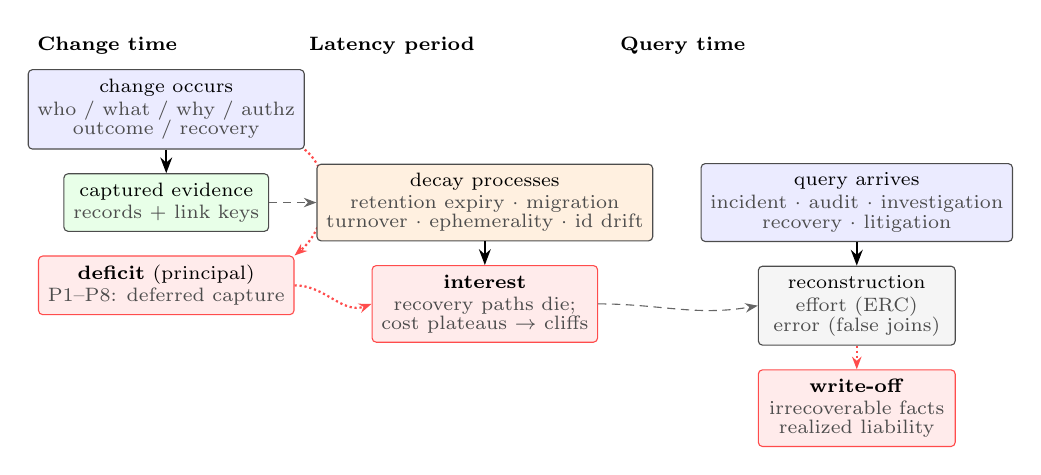
\begin{tikzpicture}[node distance=3.6mm and 4.5mm]
  % phase headers
  \node[lbl, anchor=west] (h1) at (0,0) {\textbf{Change time}};
  \node[lbl, anchor=west] (h2) at (3.45,0) {\textbf{Latency period}};
  \node[lbl, anchor=west] (h3) at (7.4,0) {\textbf{Query time}};

  % change time
  \node[human, below=3mm of h1.west, anchor=north west, minimum width=26mm] (act)
    {change occurs\\{\smlbl who / what / why / authz}\\[-1pt]{\smlbl outcome / recovery}};
  \node[attn, below=3mm of act, minimum width=26mm] (cap)
    {captured evidence\\{\smlbl records $+$ link keys}};
  \node[brok, below=3mm of cap, minimum width=26mm] (def)
    {\textbf{deficit} (principal)\\{\smlbl P1--P8: deferred capture}};
  \draw[flow] (act) -- (cap);
  \draw[bflow] (act.south east) to[out=-40,in=40] (def.north east);

  % latency
  \node[evid, right=6mm of cap, minimum width=27mm] (decay)
    {decay processes\\{\smlbl retention expiry $\cdot$ migration}\\[-1pt]{\smlbl turnover $\cdot$ ephemerality $\cdot$ id drift}};
  \node[brok, below=3mm of decay, minimum width=27mm] (interest)
    {\textbf{interest}\\{\smlbl recovery paths die;}\\[-1pt]{\smlbl cost plateaus $\to$ cliffs}};
  \draw[eflow] (cap) -- (decay);
  \draw[bflow] (def.east) to[out=0,in=200] (interest.west);
  \draw[flow] (decay) -- (interest);

  % query time
  \node[human, right=6mm of decay, minimum width=25mm] (query)
    {query arrives\\{\smlbl incident $\cdot$ audit $\cdot$ investigation}\\[-1pt]{\smlbl recovery $\cdot$ litigation}};
  \node[stage, below=3mm of query, minimum width=25mm] (rec)
    {reconstruction\\{\smlbl effort (ERC)}\\[-1pt]{\smlbl error (false joins)}};
  \node[brok, below=3mm of rec, minimum width=25mm] (wo)
    {\textbf{write-off}\\{\smlbl irrecoverable facts}\\[-1pt]{\smlbl realized liability}};
  \draw[flow] (query) -- (rec);
  \draw[bflow] (rec) -- (wo);
  \draw[eflow] (interest.east) to[out=0,in=190] (rec.west);
\end{tikzpicture}
}
\caption{The evidence-debt lifecycle. At change time, capture practices (top) either
record or defer each evidence element; deferral creates a deficit (principal). During
the latency period, decay processes---retention expiry, turnover, migration,
identifier drift---degrade the remaining reconstruction paths (interest). The debt is
realized when a query against operational history arrives (incident, audit,
investigation, recovery, litigation): surviving evidence is assembled, missing links
are reconstructed at effort cost, wrongly reconstructed at error cost, or found
irrecoverable (write-off). Boxes name the constructs formalized in
\cref{sec:definitions}.}
\label{fig:lifecycle}
\end{figure}

\Cref{fig:lifecycle} summarizes the lifecycle: creation at change time, silent
accumulation and decay during the latency period, and realization at query time.
The remainder of the paper formalizes each stage.

\section{Definitions (RQ2, Part 1)}
\label{sec:definitions}

We build the definitions in strict dependency order, so that none is circular:
syntactic objects first (schema, corpus, deficit), then operational quantities
(reconstruction cost, irrecoverability), then the economic aggregate (debt) and its
decomposition (principal, interest, liability). Each definition ends with its
\emph{observability basis}: what one would measure to instantiate it. The financial
vocabulary is used only \emph{after} the underlying quantity is defined without it.

\begin{definition}[Evidence Schema]
\label{def:schema}
An \emph{evidence schema} $\Sch$ is a declared mapping from each class of
operational change to the required set of \emph{evidence elements} for that class:
typed facts (actor identity, content delta, intent statement, authorization basis,
outcome record, recovery linkage) together with the \emph{link keys} that connect
them across stores. \emph{Observability:} $\Sch$ is an artifact the organization
writes down; its existence is a governance choice, and all subsequent measurement is
relative to it.
\end{definition}

The schema-relativity is deliberate and load-bearing: ``missing'' is undefined
without a statement of what was supposed to exist. This mirrors measurement practice
in data quality~\cite{wang1996} and avoids the circularity of defining debt by
whatever later turns out to be needed. The six-interrogative schema of
\cref{sec:schema-informal} is our reference instantiation; organizations may declare
stricter or weaker ones, and comparisons are meaningful only under a fixed $\Sch$.

\begin{definition}[Evidence Corpus]
\label{def:corpus}
The \emph{evidence corpus} $\Corp(t)$ is the set of evidence elements and link keys
that durably exist and are retrievable at time $t$, across all stores.
\emph{Observability:} enumerable by inventory of the stores, up to discoverability
limits that are themselves part of the phenomenon (\cref{sec:metrics}).
\end{definition}

\begin{definition}[Evidence Deficit]
\label{def:deficit}
For a change $x$ of class $k$ occurring at time $t_x$, the \emph{evidence deficit}
$\Def(x, t) \subseteq \Sch(k)$ is the set of schema-required elements and link keys
for $x$ absent from $\Corp(t)$. The \emph{deficit at creation} is $\Def(x, t_x)$;
elements present at $t_x$ but absent at $t > t_x$ have \emph{decayed}.
\emph{Observability:} a syntactic census---for each change, check each required
element's presence. No judgment about future cost is involved.
\end{definition}

\begin{definition}[Reconstruction and Its Cost]
\label{def:rec}
A \emph{query} $q$ against operational history asks for a set of facts and links
concerning past changes (e.g., ``what changed on service $s$ in window $w$, by whom,
under what authorization?''). \emph{Reconstruction} is the process---human,
algorithmic, or mixed---of attempting to answer $q$ from $\Corp(t)$. Its
\emph{reconstruction-attempt cost} $\ERC(q, \Corp(t))$ is the finite effort expended
(person-time and compute, on a declared accounting) until either (i) an answer of
stated confidence is reached or (ii) the declared policy stops without one. Its
\emph{error} is the divergence of any returned
answer from ground truth. Thus $\ERC$ is defined even when no answer is produced;
policy abstention and certified irrecoverability are represented separately in
\cref{def:debt,def:irrec}. \emph{Observability:} attempt cost is
measurable directly whenever reconstruction is performed (incident retrospectives,
audit preparation, the drills of \cref{sec:field}); error is measurable wherever
ground truth is independently available---natively in simulation
(\cref{sec:simulation}), partially in the field.
A \emph{reconstruction policy} $\rho$ declares the admissible sources, a finite
exhaustion rule, a confidence threshold, and the acceptance/action rule; let
$\mathcal R_q$ be the declared admissible policy class for $q$. The random variable
$C_\rho(q,E)$ is the finite effort used by policy $\rho$ on evidence $E$.
A policy is \emph{sound exhaustive} relative to $(U,\gamma,\rho_{\mathrm{exh}})$
if it completes the declared finite exhaustion and accepts an answer only when the
available evidence establishes it at confidence $\gamma$. Such a policy must
abstain at the certified irrecoverability boundary of \cref{def:irrec}.
Exhaustiveness alone does not imply soundness: an aggressive policy may inspect all
declared sources and still return $W$ after the true fact cannot be established.
Standardized drills estimate policy-specific effort by fixing $\rho$ in advance;
the total-burden optimum used for debt accounting is defined in
\cref{def:debt}, rather than by minimizing effort alone.
\end{definition}

\begin{definition}[Evidence Irrecoverability]
\label{def:irrec}
A fact or link required by query $q$ is \emph{irrecoverable relative to a declared
source universe $U$, confidence threshold $\gamma$, and exhaustion protocol
$\rho_{\mathrm{exh}}$} if no admissible procedure over
$\Corp(t)\cap U$ can establish it at confidence $\gamma$ after
$\rho_{\mathrm{exh}}$ is completed. Write this operational event as
$\Irr(q,t\mid U,\gamma,\rho_{\mathrm{exh}})$. A query is irrecoverable if any fact
essential to it is. This is a scoped certificate, not a metaphysical claim that no
forgotten backup, private message, or offline export exists anywhere.
\emph{Observability:} in simulation, exactly decidable because $U$ and ground truth
are complete; in the field, certified within an enumerated source list, as forensic
practice certifies unavailability~\cite{nist80086,casey2011}.
\end{definition}

\begin{definition}[Evidence Debt]
\label{def:debt}
Fix a schema $\Sch$, a corpus $\Corp(t)$, and a \emph{query workload} $\Qw$: a set
of potential future queries $q$ with occurrence weights $w_q > 0$ (frequencies,
probabilities, or scenario weights, declared explicitly). The default reporting
policy partitions every reconstruction outcome into exactly one of: $S$
(supported-correct), $W$ (accepted-but-wrong), or $N$ (no answer certified by
$\rho$, i.e., policy abstention).
The policy first decides an acceptance indicator $A_\rho(q,E)\in\{0,1\}$ using
only available evidence: $A_\rho=0$ implies $N$ regardless of ground truth; if
$A_\rho=1$, ground truth distinguishes $S$ from $W$. Define
$\Err_q=\{W\}$ and $\mathsf{Abst}_q=\{N\}$, so the accepted-error and policy-
abstention channels are mutually exclusive. Crucially, $\mathsf{Abst}_q$ is not
the irrecoverability event of \cref{def:irrec}: a conservative $\rho$ can abstain
while another admissible procedure could still recover the fact. Write the latter
state separately as $\mathsf I_q(E\mid U,\gamma,\rho_{\mathrm{exh}})\in\{0,1\}$.

For each query template $q$, expectations and probabilities are taken under a
declared evaluation measure $\mu_q$ over query instances and any analyst, policy,
path-survival, or seed randomness. For a deterministic single instance they reduce
to indicators; in the simulation they are empirical frequencies over the
prespecified generated instances and seeds. For a fixed policy, define
\begin{align*}
B_{q,\rho}(E)=&\;\mathbb E C_\rho(q,E)
+\lambda_q\Pr_\rho(\Err_q\mid E)\\[-2pt]
&+\pi_q\Pr_\rho(\mathsf{Abst}_q\mid E),
\end{align*}
and define the optimal total burden
\begin{align*}
B_q^{\star}(E)=\inf_{\rho\in\mathcal R_q}\bigl\{
&\mathbb E C_\rho(q,E)+\lambda_q\Pr_\rho(\Err_q\mid E)\\[-2pt]
&+\pi_q\Pr_\rho(\mathsf{Abst}_q\mid E)\bigr\}.
\end{align*}
The theoretical \emph{optimal evidence debt} of the estate at $t$ is
\begin{equation*}
\ED^{\star}(t)=\sum_{q\in\Qw}w_q
\left[B_q^{\star}(\Corp(t))-B_q^{\star}(\Corp^{*}(t))\right].
\end{equation*}
The policy-specific estimand used by a preregistered drill is instead
\begin{equation*}
\ED_{\rho}(t)=\sum_{q\in\Qw}w_q
\left[B_{q,\rho}(\Corp(t))-B_{q,\rho}(\Corp^{*}(t))\right].
\end{equation*}
Estimating $\ED^{\star}$ requires comparing multiple admissible policies or
declaring $\mathcal R_q$ a singleton; one fixed drill estimates $\ED_\rho$, not an
unobserved infimum. We use unadorned ``ED'' for the construct family and mark every
reported numerical estimate by its policy context.
When the consequence of certified physical loss must differ from a still-
recoverable abstention, replace the additive consequence terms by a declared joint
loss $L_q(Y_\rho,\mathsf I_q)$, where $Y_\rho\in\{S,W,N\}$. This permits, for
example, $L_q(N,0)\ne L_q(N,1)$ and an aggressive wrong answer with
$L_q(W,1)$, without equating a policy decision to a state of the evidence. The
additive instance above is the estimand exercised here: it prices accepted error
and policy-abstention exposure under $\rho$, while IRR is reported separately.

$\Corp^{*}(t)$ is $\Corp(t)$ augmented with every element and link key required by
$\Sch$ for every change up to $t$, captured at change time and subject to no decay.
Thus $\Corp(t)\subseteq\Corp^{*}(t)$. If every policy available on less evidence
can be emulated while ignoring extra evidence, then
$B_q^{\star}(E_2)\leq B_q^{\star}(E_1)$ whenever $E_1\subseteq E_2$; hence
$\ED^{\star}(t)\geq0$. A fixed-policy contrast $\ED_\rho$ inherits this guarantee
only if $\rho$ is information-monotone; the simulation's complete ideal corpus
resolves every link exactly at zero excess burden. This choice is deliberate and consequential: it attributes
retention- and migration-driven loss of once-captured evidence to debt (as
decay-created deficit, \cref{def:deficit}), because from the query's standpoint an
expired record and a never-captured record are the same absence with different
histories. $\lambda_q$ prices an incorrect returned answer and $\pi_q$ prices policy
abstention. Neither coefficient by itself prices certified physical
irrecoverability. \emph{Observability:} estimable, not
directly observable---the estimation problem is exactly what
\cref{sec:metrics,sec:simulation,sec:field} address; the definition fixes what the
estimators are estimators \emph{of}. In field estimation, the same preregistered
policy $\rho$ is applied to actual and ideal/reference corpora to estimate
$\ED_\rho$. In the simulation, the admissible class is the singleton accompanying
reconstructor, so $\ED_\rho=\ED^{\star}$ within that declared class.
\end{definition}

Four features of \cref{def:debt} do argumentative work. First, debt is
\emph{workload-relative}: an estate whose history will never be queried carries
deficits but little debt; declaring $\Qw$ forces the (often implicit) organizational
judgment about which contingencies matter into the open. Second, the excess-cost
form makes the baseline explicit: even a complete corpus makes queries cost
something; debt is only the part deferral added, and optimal information-monotone
total burden makes that excess nonnegative. Third, false reconstruction is priced
explicitly rather than hidden inside effort. Fourth, policy abstention is priced as
a finite consequence, while certified irrecoverability remains a separately
reported state and the mandatory physical boundary of \cref{prop:writeoff}. This
separation prevents a conservative policy from manufacturing ``irrecoverability''
merely by declining to answer.

\begin{definition}[Evidence-Debt Principal]
\label{def:principal}
The \emph{principal} of a deficit $\Def(x, t_x)$ is its contribution to $\ED(t_x)$
at creation time---the excess expected burden were the workload queried immediately,
while memory is fresh, sources are live, and identifiers are current.
\emph{Observability:} estimable at change time from the deficit census and
short-horizon reconstruction calibration.
\end{definition}

\begin{definition}[Evidence-Debt Interest]
\label{def:interest}
The \emph{interest} accrued on change $x$'s evidence position over $[t_x, t]$ is
the growth of its contribution to $\ED$ beyond principal:
$\mathcal{I}(x, t) = \mathrm{ED}\text{-contribution}(x, t) - \text{principal}(x)$.
It has two decay-driven components, both are interest, and they must not be
conflated with new borrowing: (i)~\emph{path decay}, the loss of reconstruction
routes for elements already deficient at $t_x$; and (ii)~\emph{corpus decay}, the
expiry or destruction of elements captured at $t_x$, which enlarges
$\Def(x, t)$ over time per \cref{def:deficit}. The drivers of both are the same
processes: retention expiry, record deletion, personnel
departure~\cite{rigby2016}, resource ephemerality~\cite{burns2016}, identity and
schema drift, vendor migration, and loss of correlation identifiers.
\emph{Observability:} the decay processes are individually observable (retention
policies are published~\cite{cloudtrail,ghdocs,nist80092}; turnover is known to HR;
migrations are scheduled); \cref{sec:interest} shows how their superposition yields
a computable burden-versus-age curve, and why it is not a compound rate.
Interest is gross decay-driven accrual in the absence of remediation. Backfill and
restored linkage are repayments that reduce the debt stock; they are not negative
interest.
\end{definition}

\begin{definition}[Evidence Liability]
\label{def:liability}
The \emph{liability} of the estate with respect to a specific contingency $q$ at $t$
is the conditional realized burden if $q$ occurs at $t$: the actual reconstruction
cost plus the consequence cost of wrongly answered parts or parts left uncertified
by $\rho$ (regulatory
exposure, prolonged outage, lost claims)~\cite{sedona2018,sox2002}.
\emph{Observability:} realized liabilities are observable events (audit findings,
incident duration attributable to archaeology); $\ED$ is their workload-weighted
expectation, which is the standard relation between an expected cost and its
realizations.
\end{definition}

\begin{figure}[t]
\centering
\resizebox{0.70\columnwidth}{!}{% Accounting bridge from evidence deficit to financial exposure (single column)
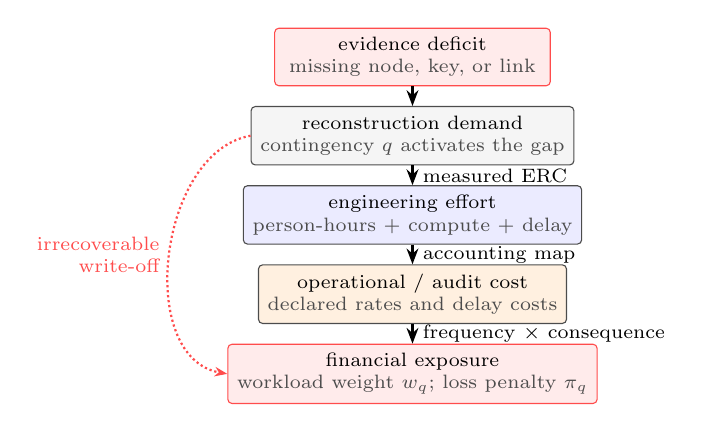
\begin{tikzpicture}[node distance=2.5mm]
  \node[brok, minimum width=35mm] (deficit)
    {evidence deficit\\{\smlbl missing node, key, or link}};
  \node[stage, below=of deficit, minimum width=35mm] (recon)
    {reconstruction demand\\{\smlbl contingency $q$ activates the gap}};
  \node[human, below=of recon, minimum width=35mm] (hours)
    {engineering effort\\{\smlbl person-hours $+$ compute $+$ delay}};
  \node[evid, below=of hours, minimum width=35mm] (cost)
    {operational / audit cost\\{\smlbl declared rates and delay costs}};
  \node[brok, below=of cost, minimum width=35mm] (exposure)
    {financial exposure\\{\smlbl workload weight $w_q$; loss penalty $\pi_q$}};

  \draw[flow] (deficit) -- (recon);
  \draw[flow] (recon) -- node[right,lbl]{measured ERC} (hours);
  \draw[flow] (hours) -- node[right,lbl]{accounting map} (cost);
  \draw[flow] (cost) -- node[right,lbl]{frequency $\times$ consequence} (exposure);
  \draw[bflow] (recon.west) to[out=190,in=170]
    node[left,lbl,align=right]{irrecoverable\\write-off} (exposure.west);
\end{tikzpicture}
}
\caption{The causal accounting bridge from a syntactic deficit to economic
exposure. Only the first node is obtained by census. Reconstruction drills
measure ERC; declared labor, compute, and delay rates map effort to cost; workload
weights and accepted-error/abstention penalties map policy outcomes to exposure;
physical irrecoverability remains a separate loss state. The figure
defines an auditable chain, not a claim that this paper has estimated dollars.}
\label{fig:economic-chain}
\end{figure}

\Cref{fig:economic-chain} makes explicit the economic bridge that the excess-cost
definition otherwise compresses into one term. A deficit has no intrinsic monetary
value. It becomes economically relevant only when a contingency demands
reconstruction; the resulting person-time, compute, and delay can then be mapped
through published accounting rates, and the workload weights and consequence
penalties of \cref{def:debt} turn those conditional costs into exposure. This
separation is intentional: the paper can define and measure reconstruction burden
without pretending to have measured wages, outage revenue, or regulatory loss.

The resulting vocabulary is internally consistent and independent of the financial
metaphor: \emph{deficit} is syntax (what is missing),
\emph{debt} is expectation (the excess reconstruction effort, accepted error, and
policy abstention the missing evidence is expected to cause),
\emph{principal} is the at-creation component, \emph{interest} is the decay-driven
growth, \emph{liability} is the per-contingency realization, and
\emph{irrecoverability} is the terminal physical loss state, priced separately only
through a declared joint loss when policy abstention is not an adequate proxy.
\Cref{sec:model} gives the machinery that connects them.

\section{A Formal Model of Evidence Debt (RQ2--RQ4)}
\label{sec:model}

The definitions of \cref{sec:definitions} refer to reconstruction cost and decay
without structure. This section supplies the structure: operational history as a
graph, evidence as a fragmented projection of it, reconstruction as linkage
inference, and decay as survival processes over sources. The model is chosen so that
every parameter is either directly observable or estimable by the procedures of
\cref{sec:metrics,sec:field}, and so that the qualitative predictions tested in
\cref{sec:simulation} follow from it rather than from intuition.

\subsection{History, Evidence, and Fragmentation}
\label{sec:model-graph}

\textbf{Ground truth.} Operational history is a typed, acyclic \emph{event graph}
$\Hist = (V, L)$: nodes $V$ are events and artifacts of a change (intent record,
content revision, authorization act, build, artifact, deployment, runtime
configuration, outcome), and links $L \subseteq V \times V$ are the true causal and
derivational relations among them. A \emph{chain} is the subgraph of one logical
change. $\Hist$ is what actually happened; no one holds it directly.

\textbf{Evidence.} The corpus $\Corp(t)$ (\cref{def:corpus}) is a set of
\emph{records}, each held in a store $s \in S$, each testifying to a node and
carrying zero or more \emph{link keys}: identifiers intended to name adjacent nodes
(a ticket id in a commit message, a commit hash in a build record, a digest in a
deployment record)~\cite{sigelman2010}. The corpus thus determines an
\emph{observed graph}: nodes for surviving records, and an edge wherever a surviving
key names a surviving record. Fragmentation is the model's default: records of one
chain are distributed across stores with independent schemas, clocks, and retention
regimes (\cref{sec:amplifiers}).

\textbf{Deficit classes.} Relative to schema $\Sch$, a deficit
(\cref{def:deficit}) is one of: a \emph{missing node} (the record never existed or
was deleted), a \emph{missing key} (the record exists but the link key was never
propagated or was stripped), or a \emph{degraded attribute} (e.g., a null timestamp,
an unresolvable identity). The distinction is not pedantic: \cref{sec:simulation}
shows missing nodes and missing keys have different cost signatures---keys are
compensable by inference at effort-and-error cost; nodes, once every copy is gone,
are not compensable at all.

\subsection{Reconstruction as Linkage Inference}
\label{sec:model-linkage}

A query $q$ (\cref{def:rec}) requires recovering a subset of true links $L_q$. Where
keys survive, recovery is lookup. Where they do not, recovery is \emph{record
linkage}: deciding, from attributes (service, actor, temporal proximity, content
similarity), which surviving records refer to adjacent events---precisely the
inference problem formalized by Fellegi and Sunter~\cite{fellegi1969} and developed
in entity resolution~\cite{christen2012}. This identification imports the right
consequences. Linkage has \emph{effort}: candidate sets must be enumerated and
compared, and effort grows with the ambient density of similar records. Linkage has
\emph{error}: with imperfect discriminators, some accepted matches are false; false
links do not announce themselves, so the reconstructed history is silently wrong.
And linkage has \emph{limits}: when discriminating attributes are themselves
degraded (timestamps nulled, identities recycled), candidates become
indistinguishable and links unrecoverable even though both endpoint records
survive.

For a single required link $\ell$, let $\mathrm{paths}(\ell, t)$ be its surviving
\emph{recovery paths} at $t$: the direct key, redundant keys (a digest recorded in
two places), inferential linkage over attributes, and extra-corpus paths (asking the
engineer who did it). Each path $r$ has expected effort $c_r(t)$ and error rate
$\varepsilon_r(t)$. Under a fixed confidence-threshold policy, the effort-minimizing
acceptable path gives the link cost
\[
c_\ell(t) \;=\; \min \{\, c_r(t) : r \in \mathrm{paths}(\ell, t),\;
\varepsilon_r(t) \le \bar{\varepsilon} \,\},
\]
with $c_\ell(t)$ undefined---the link irrecoverable (\cref{def:irrec})---when the
set is empty. This path-level minimum is the cost of obtaining an acceptable answer,
not the always-finite attempt cost $\ERC$ of \cref{def:rec}. For an irrecoverable
link, $\ERC$ instead includes the finite search needed to exhaust the declared source
set and certify failure; $\mathsf I_q$ records the resulting physical loss state.
Policy abstention $\mathsf{Abst}_q$ can occur earlier and is not evidence that this
exhaustion boundary has been reached. For recoverable
links, query attempt cost aggregates the selected path costs (with shared-work
economies we do not model further). A returned link inconsistent with ground truth
sets $\Err_q$; the $\lambda_q$ term of \cref{def:debt} is therefore what makes
false reconstruction part of the debt quantity rather than merely a diagnostic
beside it. More generally, $B_q^{\star}$ in \cref{def:debt} minimizes the joint
effort, accepted-error, and abstention burden over admissible policies; it need
not choose the effort-minimizing path when a more expensive path reduces expected
consequence loss. $\ED^{\star}(t)$ compares optimal total burden with the ideal
corpus; $\ED_\rho(t)$ makes the same comparison for a fixed policy.

\subsection{Why Not $ED = f(M, F, R, U, C)$}
\label{sec:model-notformula}

A natural first proposal---and the one we expect readers to reach for---is a form
$ED = f(M, F, R, U, C)$ over missingness, fragmentation, retention risk,
uncertainty, and reconstruction cost. We considered and declined the form, keeping
the factors. The
reason is that the five quantities are not independent inputs to be aggregated; they
occupy different roles in the mechanism. Missingness ($M$) parameterizes the
deficit census. Fragmentation ($F$) and correlation uncertainty ($U$) shape the
\emph{cost and error of inferential paths}: fragmentation multiplies the stores to
be searched, and $U$---driven by ambient record density and discriminator
quality---sets false-match rates~\cite{fellegi1969}. Retention risk ($R$) is a
property of \emph{decay}: it determines which paths survive to time $t$
(\cref{sec:model-decay}). Reconstruction cost ($C$) is not an input at all; it is
the \emph{output} the others produce through the path structure. A scalar
aggregation of the five would assign weights to quantities whose interaction is
mediated by minimization over paths---and the minimization is what generates the
phenomena that matter (plateaus, cliffs, superadditivity; \cref{sec:model-props}).
Any composite index built for reporting purposes (\cref{met:edi}) must therefore be
understood as an estimator of \cref{def:debt}, not as its definition.

\subsection{Decay: Survival of Recovery Paths}
\label{sec:model-decay}

Each recovery path $r$ for a link has a \emph{survival function}
$\surv_r(\tau)$: the probability it remains usable $\tau$ after chain creation. The
empirically dominant forms are: \emph{step survival} for policy-driven retention
(a CI log is present until day $T_r$, then gone~\cite{nist80092,ghdocs,
cloudtrail}); \emph{event survival} for migrations and decommissionings (present
until an organizational event at an uncertain date); \emph{hazard survival} for
human sources (available until the holder departs, with turnover hazard
$\haz$~\cite{rigby2016}); and \emph{drift degradation} for inferential paths
(discriminators weaken as identities are recycled and schemas
evolve~\cite{parnas1994,lehman1980}). Interest (\cref{def:interest}) is the
consequence: as paths die, $c_\ell(t)$ jumps to the next-cheapest survivor, and
when the last dies, the link crosses into irrecoverability.

\subsection{Propositions}
\label{sec:model-props}

The following are analytic consequences of the path model; proofs are elementary
and stated to make the dependency structure explicit. Their empirical counterparts
are exercised in \cref{sec:simulation}, which distinguishes design-entailed
demonstrations from the falsifiable tests (notably the pairwise interaction test
of \cref{prop:superadd}).

\begin{proposition}[Effort plateau under a fixed acceptance policy]
\label{prop:plateau}
If a link retains at least one surviving path whose cost equals the original
cheapest cost, its expected reconstruction cost is unchanged by the loss of any
number of other paths. Consequently, estate-level cost as a function of a
degradation rate is flat while redundancy lasts and departs from flatness only as
cheapest paths begin to be destroyed. No plateau claim follows for total burden
unless a surviving path also preserves the error and consequence profile of the
previously burden-optimal policy.
\end{proposition}
\begin{proof}
Immediate from $c_\ell = \min$ over surviving paths: the minimum is invariant to
removal of non-minimal elements.
\end{proof}

\begin{proposition}[Superadditive interaction of deficit classes]
\label{prop:superadd}
Let two degradation classes each destroy a disjoint subset of paths such that
neither alone destroys any link's full path set. Then each alone adds bounded
effort cost and zero irrecoverability, while their combination can make the link
irrecoverable. The irrecoverability indicator is therefore strictly superadditive
for that link; no corresponding claim about the effort component or total $\ED$
follows without additional cost inequalities.
\end{proposition}
\begin{proof}
By construction, irrecoverability requires the surviving-path set to be empty
(\cref{def:irrec}). If class $A$ leaves $P \setminus A$ nonempty and class $B$
leaves $P \setminus B$ nonempty, but $A \cup B \supseteq P$, then
$\Irr_\ell(A)=\Irr_\ell(B)=0$ and $\Irr_\ell(A\cup B)=1$. Hence $1>0+0$.
For a sound exhaustive policy the combination also forces abstention. Under another
policy, physical irrecoverability may coexist with $W$ or $N$. In every case the
physical state is distinct from the policy decision and introduces no undefined or
infinite reconstruction cost.
\end{proof}

\begin{proposition}[Effort plateau and irrecoverability cliff]
\label{prop:steps}
Under the survival forms of \cref{sec:model-decay}, the expected finite
reconstruction-attempt cost of a fixed deficit is piecewise: constant
while the cheapest surviving path persists, jumping at retention boundaries and
organizational events, with smooth growth only where a hazard-governed human path
is the cheapest survivor. When the last answer-producing path dies, the remaining
cost is the finite effort of certifying irrecoverability. Under a sound exhaustive
policy, abstention then switches on and coincides with the physical loss state;
under a conservative policy it may switch on earlier, while an unsound or
aggressive policy may instead return $W$. The error and
abstention components have the same plateau-and-cliff form only when path error and
the acceptance rule remain constant between degradation events; in general they
change as discriminators degrade. Thus no constant $\rho$ makes total burden grow as
$e^{\rho \tau}$ in general.
\end{proposition}
\begin{proof}
Piecewise-constancy between path deaths follows from \cref{prop:plateau}; jumps at
step/event survival boundaries follow from minimization passing to the next
survivor, or to finite source-exhaustion effort when none remains; the only smooth
component is the expectation over hazard-distributed death times of a human path,
which yields growth bounded by the next attempt state's cost, not unbounded
compounding.
Error burden follows the same argument only under the stated between-event
constant-error assumption; otherwise its shape is determined by discriminator
degradation.
\end{proof}

\begin{proposition}[Bounded burden; mandatory irrecoverability boundary]
\label{prop:writeoff}
With finite penalty weights $\lambda_q$ and $\pi_q$, $\ED^{\star}(t)$ (and any
finite policy-specific $\ED_\rho(t)$) is bounded above by
$\sum_q w_q(\bar{C}_q + \max\{\lambda_q,\pi_q\})$, where $\bar{C}_q$ is the cost of $q$'s most
expensive reconstruction-attempt state. Once a link is irrecoverable, further decay
cannot restore an answer-producing path; the finite certification effort remains
bounded by $\bar{C}_q$. At physical irrecoverability, a sound exhaustive policy must
abstain; another policy may incur accepted-error burden instead. In all cases the
burden remains finite and does not grow without bound; it reaches a realized loss
cap. Financial debt has no
analogous physical write-off boundary imposed by the world rather than chosen by a
creditor.
\end{proposition}
\begin{proof}
Directly from \cref{def:debt}: reconstruction-attempt cost is finite by
\cref{def:rec} and bounded here by $\bar{C}_q$, while each probability difference
is at most one. Each query's contribution is therefore at most
$w_q(\bar{C}_q+\max\{\lambda_q,\pi_q\})$, because the default policy's accepted-
error and abstention outcomes are mutually exclusive.
\end{proof}

\label{sec:model-anti}
\Cref{prop:steps,prop:writeoff} are the model's verdict on the metaphor, obtained
before any experiment: evidence debt has principal and carrying cost, but its
effort and abstention exposure under sound exhaustive policies are stochastic,
discontinuous, and driven by third
parties' retention clocks rather than by any contracted rate; error exposure can
also drift continuously as discriminators weaken. Answerability terminates at a
physical write-off boundary rather than compounding indefinitely.
\Cref{sec:disc-metaphor} completes the
argument that the constructs stand without the metaphor.

\begin{proposition}[Measurement reduction]
\label{prop:reduction}
$\ED^{\star}(t)$ is determined by four input families: (i)~the deficit/corpus census
(observable, \cref{def:deficit}); (ii)~the reconstruction protocol family,
including admissible policies, confidence and finite-exhaustion rules, and
per-path effort/error calibrations; (iii)~the survival schedule of paths
(observable from retention policies, HR data, and migration calendars); and
(iv)~the declared workload and consequence weights $(w_q,\lambda_q,\pi_q)$.
\end{proposition}
\begin{proof}
By inspection of \cref{def:debt} through \cref{sec:model-linkage,sec:model-decay}:
the expectation is over path survival (iii), applied through the declared
reconstruction protocols (ii) to the corpus described by (i), and aggregated
under (iv).
\end{proof}

Two honesty notes bound what \cref{prop:reduction} claims. First, it is an
input-enumeration result, not a feasibility result: input (ii)---per-path cost and
error calibrations for future queries---is the empirically hard part, obtainable
only by reconstruction drills (\cref{sec:field}) and bounded, not supplied, by
linkage theory~\cite{fellegi1969}. Second, inputs (i) and (iv) are relative to
declared governance choices ($\Sch$; $w_q, \lambda_q, \pi_q$), so $\ED$ values are
comparable across estates only under shared reference declarations
(\cref{sec:metrics,sec:disc-relativity}). RQ2 is therefore answered as:
\emph{quantifiable relative to declared governance inputs, with the empirical
burden concentrated in cost calibration}---an affirmative with stated conditions,
not an unconditional one. \Cref{sec:metrics} turns the inputs into named metrics;
\cref{sec:sim-workload} instantiates the entire chain, computing $\ED_\rho(t)$ end to end in
a closed world where every input is known.

\section{Metrics: Proposal and Critical Evaluation (RQ2, Part 2)}
\label{sec:metrics}

We evaluate six candidate metrics---and commit in advance to rejecting any that
cannot be justified---against three criteria: \emph{grounding}
(does it estimate a quantity of \cref{sec:definitions,sec:model}?),
\emph{operationalizability} (can it be computed from obtainable data?), and
\emph{incentive safety} (what does optimizing it do?). One candidate is rejected;
one is accepted only with a replacement semantics; the remainder are adopted with
stated scope. The foundational metrics (EDR analogues, ERC/FRR/AR reconstruction performance,
irrecoverability, and $\ED$ itself) are computed concretely in
\cref{sec:simulation}; the replacement decay-schedule semantics is computed in
\cref{sec:interest}; the flow metric (M4) and the composite (M6) are defined for
field use and not exercised here.

\begin{metricdef}[Evidence Deficit Ratio, EDR]
\label{met:edr}
For an estate and schema $\Sch$: the fraction of schema-required elements and link
keys absent from the corpus, reported per deficit class (missing node, missing key,
degraded attribute) and per interrogative (who/what/why/authorization/outcome/%
recovery). \emph{Verdict: adopted.} Grounded directly in \cref{def:deficit};
computable by automated census; class-resolved reporting resists the false comfort
of a single number. This is the suite's foundation metric---syntactic, cheap, and
continuously monitorable.
\end{metricdef}

\begin{metricdef}[Evidence Reconstruction Performance, ERC, FRR, and AR]
\label{met:erc}
The triplet comprising (i)~Evidence Reconstruction Cost (ERC): measured person-time,
compute, or calendar latency for a defined query; and (ii)~False Reconstruction
Rate (FRR): the fraction of accepted facts or links that diverge from independent
ground truth; and (iii)~policy Abstention Rate (AR): the fraction for which $\rho$
certifies no answer. All are measured under the same preregistered confidence and
acceptance policy, per \cref{def:rec}, and collected from
real reconstructions (incidents, audits) or standardized drills (\cref{sec:field});
in simulation, effort is proxied by candidate comparisons and FRR is scored exactly.
\emph{Verdict: adopted.} The triplet exposes the effort--accuracy--abstention
tradeoff that ERC alone can hide. AR is not IRR: the former is a policy outcome,
the latter a certified evidence state.
\end{metricdef}

\begin{metricdef}[Irrecoverability Ratio, IRR]
\label{met:irr}
The fraction of a defined query set (or of required links) irrecoverable at $t$
within a published $(U,\gamma,\rho_{\mathrm{exh}})$ declaration, per
\cref{def:irrec}. \emph{Verdict: adopted.} Decidable exactly in simulation;
certifiable in the field by source-exhaustion protocols~\cite{nist80086}. Reported
separately from cost metrics because it measures loss, not effort, and the two must
never be averaged together (\cref{prop:writeoff}).
\end{metricdef}

\begin{metricdef}[Evidence Debt Inflow Rate, EDIR]
\label{met:growth}
The inflow attributable to \emph{new} deficit creation per unit time:
in practice, the deficit-census delta per unit time (new changes arriving with
incomplete evidence), weighted by principal estimates. \emph{Verdict: adopted.}
This measures the inflow (are we borrowing faster?), and must
be reported separately from interest accrual on the existing stock; conflating the
two makes remediation invisible. The net stock change is instead
$d\ED/dt=\text{inflow}+\text{decay accrual}-\text{repayment}
-\text{write-off realization}$.
\end{metricdef}

\begin{metricdef}[Evidence-Debt Interest Rate]
\label{met:interest}
\emph{Proposed as}: a scalar rate $\rho$ such that reconstruction cost grows as
$e^{\rho\tau}$ or linearly at rate $\rho$. \emph{Verdict: rejected.}
\Cref{prop:steps} shows that growth in effort and abstention exposure under sound
exhaustive policies is schedule-driven and generally
piecewise, while error depends on discriminator degradation; neither supports a
single invariant rate. Any fitted scalar is an artifact of the observation window and
extrapolates falsely across retention cliffs. \emph{Replacement:} the
\textbf{decay schedule} of the estate---the dated sequence of upcoming path-death
events (retention expirations, migrations, projected turnover quantiles) with the
cost jump each implies---and, where a single summary is required, the
\textbf{evidence half-life}: the age $\tau_{1/2}$ at which half of a reference
query set ceases to be answerable at baseline cost. Both are computable from the
survival inventory (\cref{prop:reduction}) and are demonstrated in
\cref{sec:interest}.
\end{metricdef}

\begin{metricdef}[Evidence Debt Index, EDI]
\label{met:edi}
A composite scalar summarizing estate debt for management reporting: a weighted
aggregation of EDR (by interrogative), calibrated ERC, false-reconstruction
exposure (FRR priced by $\lambda_q$), abstention exposure (AR priced by $\pi_q$),
projected decay from the decay schedule, and separately reported IRR, with published
weights. \emph{Verdict: adopted with explicit estimator
status and health warnings.} By \cref{sec:model-notformula}, any such composite is
a policy-specific estimator related to $\ED_\rho$ under assumptions, not a
definition of $\ED^{\star}$;
its weights encode the workload judgment $(w_q, \lambda_q, \pi_q)$ and must be published for
any comparison; and it inherits the gaming risks of all composites---optimizing EDI
by weakening the schema $\Sch$ is the exact analogue of declaring bankruptcy
solvent by redefining assets. EDI is defensible only alongside the disaggregated
vector (EDR by class, measured ERC/FRR/AR, decay schedule, and IRR).
\end{metricdef}

Two measurement caveats apply to the whole suite. \emph{Discoverability bias}: the
census can only inspect stores it knows about; evidence in unknown stores is
neither counted as present nor as deficit---field deployments should treat store
discovery as part of the census. \emph{Confidence accounting}: reconstructed
answers vary in confidence; ERC and FRR must be reported under the same stated
confidence and acceptance policy, or performance is not comparable. The simulation sidesteps both (closed
world, exact scoring); the field protocol confronts them directly
(\cref{sec:field}).

\section{Simulation Study: Controlled Evidence Degradation (RQ3, RQ4)}
\label{sec:simulation}

We now exercise the framework in the one setting where ground truth is available
by construction: a synthetic estate whose complete history is generated, then
degraded under experimental control. The study is executed, not merely designed;
every number below was produced by the released artifact ($\approx$560 lines of
dependency-free Python), is deterministic given the published seeds, and the
results table is generated programmatically from the run outputs. Its epistemic
role is stated with care, because a simulation whose apparatus is written by the
authors of the model cannot ``confirm'' claims that the apparatus embodies.
We therefore separate, explicitly, (i)~\emph{demonstrations}: behaviors entailed
by design choices that mirror real toolchains, whose value is quantification and
whose evidential force is tested by \emph{removal arms} in which the choice is
switched off; and (ii)~\emph{falsifiable tests}: predictions that the apparatus
does not build in and that the data could have refuted. The study validates
construct computability end to end---including $\ED(t)$ itself
(\cref{sec:sim-workload})---and estimates no real-world magnitudes.

\subsection{Apparatus}
\label{sec:sim-apparatus}

\begin{figure}[t]
\centering
\resizebox{\columnwidth}{!}{% Degradation experiment pipeline (single column, resized)
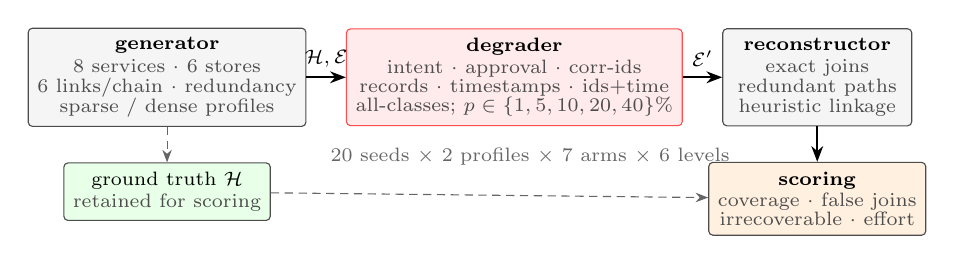
\begin{tikzpicture}[node distance=3.6mm and 5mm]
  \node[stage, minimum width=24mm] (gen)
    {\textbf{generator}\\{\smlbl 8 services $\cdot$ 6 stores}\\[-1pt]{\smlbl 6 links/chain $\cdot$ redundancy}\\[-1pt]{\smlbl sparse / dense profiles}};
  \node[brok, right=of gen, minimum width=24mm] (deg)
    {\textbf{degrader}\\{\smlbl intent $\cdot$ approval $\cdot$ corr-ids}\\[-1pt]{\smlbl records $\cdot$ timestamps $\cdot$ ids+time}\\[-1pt]{\smlbl all-classes; $p \in \{1,5,10,20,40\}\%$}};
  \node[stage, right=of deg, minimum width=24mm] (rec)
    {\textbf{reconstructor}\\{\smlbl exact joins}\\[-1pt]{\smlbl redundant paths}\\[-1pt]{\smlbl heuristic linkage}};
  \draw[flow] (gen) -- node[lbl, above]{$\Hist,\Corp$} (deg);
  \draw[flow] (deg) -- node[lbl, above]{$\Corp'$} (rec);

  \node[attn, below=4.5mm of gen, minimum width=24mm] (truth)
    {ground truth $\Hist$\\{\smlbl retained for scoring}};
  \node[evid, below=4.5mm of rec, minimum width=24mm] (score)
    {\textbf{scoring}\\{\smlbl coverage $\cdot$ false joins}\\[-1pt]{\smlbl irrecoverable $\cdot$ effort}};
  \draw[eflow] (gen) -- (truth);
  \draw[flow] (rec) -- (score);
  \draw[eflow] (truth) -- (score);
  \node[lbl, below=1.5mm of deg, xshift=2mm, text=black!60]
    {20 seeds $\times$ 2 profiles $\times$ 7 arms $\times$ 6 levels};
\end{tikzpicture}
}
\caption{The evidence-degradation experiment. A generator emits a complete
synthetic estate (ground-truth chains and their records across six stores); a
degrader removes a controlled fraction $p$ of one or more evidence classes; an
algorithmic reconstructor rebuilds each chain from surviving records (exact key
joins, then redundant-key paths, then heuristic linkage); scoring against ground
truth yields coverage, false joins, two irrecoverability constructs, invariant
effort, and $\ED$ under a declared workload.}
\label{fig:experiment}
\end{figure}

\subsubsection{Ground truth}
Each run generates an estate of eight services whose changes produce six-record
chains across six stores---ticket (ITSM), commit (forge), approval (review),
build (CI), artifact (registry), deployment (CD), plus the runtime configuration
record serving as query entry point---linked by the keys real toolchains use.
Six ground-truth links per chain instantiate the six interrogatives. The
generator includes \emph{redundancy} (the artifact digest recorded in both build
and configuration records), mirroring practice; because this choice matters, a
removal arm disables it (\cref{sec:sim-sensitivity}). Inter-record time gaps are
drawn below the reconstructor's default heuristic window; a removal arm breaks
that relationship too.

\subsubsection{Factors and arms}
The main factorial crosses \emph{degradation class}---intent links, approval
links, correlation identifiers, whole-record deletion, timestamps, the
\emph{pairwise} arm (correlation identifiers $+$ timestamps, which instantiates
the premise of \cref{prop:superadd}: neither class alone destroys records), and
an \emph{all-classes} arm---with \emph{level}
$p \in \{0,1,5,10,20,40\}\%$ and \emph{activity profile} (sparse: 50
chains/service, 180 days, 12 actors; dense: 150 chains/service, 90 days, 6
actors), 20 seeds per cell. Sensitivity arms (\cref{sec:sim-sensitivity}) vary
one design choice at a time: heuristic window below the maximum true gap;
redundancy off; ticket filer $\ne$ commit author for 30\% of chains; and a
single-knob density sweep (chains/service $\in \{50,100,150\}$ with actor pool
and window fixed), the latter because the sparse/dense profiles deliberately
bundle three knobs and cannot isolate density.

\subsubsection{Reconstructor and invariant effort accounting}
For each configuration record, the reconstructor rebuilds the chain backward:
surviving exact keys and redundant key paths first (implemented as index
lookups and charged \emph{zero} effort, so that effort does not depend on
incidental data-structure choices), then heuristic linkage (same-service
candidates within a 48-hour window, actor agreement where applicable; unique
candidate accepted; multiple candidates resolved nearest-in-time---a realistic
policy that can produce \emph{false joins}). Effort is counted only at
heuristic decision points, as two implementation-invariant quantities: the
number of links requiring non-exact resolution (\emph{fallback links}) and the
candidate records examined there.

\subsubsection{Scoring: two irrecoverability constructs}
Against ground truth we score \emph{link coverage}, \emph{false-join rate}
(incorrect/accepted), \emph{chain coverage}, and two distinct irrecoverability
constructs whose separation \cref{sec:model-graph} demands: \emph{record loss}
(a required record exists in no store---the destroyed-source clause of
\cref{def:irrec}) and \emph{identifiability-based irrecoverability}
(\cref{def:irrec} in full: record destroyed, \emph{or} no key path survives and
the discriminators---timestamps, actor, service, window---fail to single out
the true parent). The second is decidable here because the closed world knows
the truth; it is the construct the definition means, and it behaves very
differently from record loss (\cref{fnd:constructs}). One scoring asymmetry is
noted for reusers: five links are scored on the recovered parent's key, while
the approval link---whose evidential record sits on the child side---is scored
on the approval record's key; the artifact documents the orientation.

\subsubsection{$\ED$ under a declared workload}
\label{sec:sim-workload}
To instantiate \cref{def:debt} end to end, we declare a synthetic workload: one
full-chain audit query per running configuration, unit weight; resolution cost
$= 1$ unit per fallback link $+\,0.01$ per candidate examined; write-off
penalty $\pi = 50$ units per identifiability-irrecoverable link. The complete
corpus $\Corp^{*}$ resolves every link exactly, so its cost is zero and
measured cost is excess cost. The declarations are arbitrary in magnitude and
declared precisely because \cref{def:debt} requires them---the point is the
demonstrated pipeline from census to a computed $\ED(t)$, and the sensitivity
of $\ED$'s composition to the declarations is itself a result
(\cref{fnd:ed}).

\subsection{Demonstrations, Predictions, and Results}
\label{sec:sim-results}

\begin{table*}[t]
\centering
\caption{Selected Results, Generated Programmatically from the Run Outputs\\(Mean over 20 Seeds; SD in Parentheses). Cov = Link Coverage,\\FJ = False-Join Rate, Irr = Identifiability-Based Irrecoverable Chains,\\FB = Fallback Links per Chain, ED = Computed Debt (Units, \Cref{sec:sim-workload})}
\label{tab:results}
\footnotesize
\begin{tabular}{@{}llrlllll@{}}
\toprule
\textbf{Class} & \textbf{Prof.} & $p$ & \textbf{Cov} & \textbf{FJ} & \textbf{Irr} & \textbf{FB} & \textbf{ED} \\
\midrule
combined & sparse & 0\% & 1.000 (0.000) & 0.000 (0.000) & 0.000 (0.000) & 0.00 (0.00) & 0.0 (0.0) \\
combined & dense & 0\% & 1.000 (0.000) & 0.000 (0.000) & 0.000 (0.000) & 0.00 (0.00) & 0.0 (0.0) \\
intent links & dense & 40\% & 0.991 (0.001) & 0.009 (0.001) & 0.168 (0.011) & 0.40 (0.01) & 9.4 (0.6) \\
approval links & dense & 40\% & 0.953 (0.002) & 0.047 (0.002) & 0.401 (0.015) & 0.40 (0.01) & 21.1 (0.8) \\
correlation ids & dense & 40\% & 0.840 (0.010) & 0.160 (0.010) & 0.653 (0.013) & 0.97 (0.03) & 49.1 (1.3) \\
timestamps & dense & 40\% & 1.000 (0.000) & 0.000 (0.000) & 0.000 (0.000) & 0.00 (0.00) & 0.0 (0.0) \\
ids plus timestamps & dense & 40\% & 0.648 (0.011) & 0.180 (0.007) & 0.651 (0.012) & 0.86 (0.02) & 47.9 (1.3) \\
source artifacts & sparse & 40\% & 0.332 (0.012) & 0.266 (0.020) & 0.954 (0.010) & 1.41 (0.04) & 145.9 (4.0) \\
source artifacts & dense & 40\% & 0.323 (0.009) & 0.612 (0.009) & 0.953 (0.008) & 2.09 (0.07) & 147.5 (1.8) \\
combined & sparse & 5\% & 0.866 (0.015) & 0.058 (0.012) & 0.318 (0.025) & 0.42 (0.03) & 24.0 (1.9) \\
combined & dense & 5\% & 0.839 (0.008) & 0.145 (0.008) & 0.355 (0.015) & 0.44 (0.02) & 27.0 (1.3) \\
combined & sparse & 20\% & 0.530 (0.017) & 0.137 (0.013) & 0.837 (0.016) & 1.25 (0.04) & 97.5 (3.5) \\
combined & dense & 20\% & 0.502 (0.011) & 0.384 (0.010) & 0.872 (0.009) & 1.57 (0.05) & 105.6 (2.2) \\
combined & sparse & 40\% & 0.231 (0.013) & 0.145 (0.019) & 0.990 (0.006) & 1.43 (0.04) & 186.8 (3.2) \\
combined & dense & 40\% & 0.234 (0.008) & 0.479 (0.019) & 0.992 (0.002) & 1.98 (0.06) & 191.2 (2.0) \\
\bottomrule
\end{tabular}

\end{table*}

\begin{figure*}[t]
\centering
% Simulation results, 2x2 group (two-column width), data from data/series/
\begin{tikzpicture}
\begin{groupplot}[
  group style={group size=2 by 2, horizontal sep=1.55cm, vertical sep=1.45cm},
  edplot,
]
% (a) coverage, dense
\nextgroupplot[title={(a) link coverage (dense)}, ylabel={coverage},
  ymin=0, ymax=1.05, legend pos=south west]
\addplot[serA, mark=*, mark size=1.5pt, thick]
  table[x=p, y=cov, col sep=comma] {data/series/dense_approval_links.csv};
\addlegendentry{approval links}
\addplot[serC, mark=square*, mark size=1.4pt, thick, densely dashed]
  table[x=p, y=cov, col sep=comma] {data/series/dense_correlation_ids.csv};
\addlegendentry{correlation ids}
\addplot[black, mark=pentagon*, mark size=1.6pt, thick]
  table[x=p, y=cov, col sep=comma] {data/series/dense_ids_plus_timestamps.csv};
\addlegendentry{ids $+$ timestamps (pairwise)}
\addplot[serB, mark=triangle*, mark size=1.8pt, thick, dash dot]
  table[x=p, y=cov, col sep=comma] {data/series/dense_source_artifacts.csv};
\addlegendentry{record deletion}
\addplot[serD, mark=diamond*, mark size=1.8pt, thick, densely dotted]
  table[x=p, y=cov, col sep=comma] {data/series/dense_combined.csv};
\addlegendentry{all classes}

% (b) false joins, combined, both profiles
\nextgroupplot[title={(b) false-join rate (all-classes arm)},
  ylabel={false joins / accepted links}, ymin=0, ymax=0.55,
  legend pos=north west]
\addplot[serD, mark=diamond*, mark size=1.8pt, thick]
  table[x=p, y=false, col sep=comma] {data/series/dense_combined.csv};
\addlegendentry{dense}
\addplot[serA, mark=o, mark size=1.5pt, thick, densely dashed]
  table[x=p, y=false, col sep=comma] {data/series/sparse_combined.csv};
\addlegendentry{sparse}

% (c) irrecoverability constructs
\nextgroupplot[title={(c) irrecoverability constructs (dense)},
  ylabel={fraction of chains}, ymin=0, ymax=1.05, legend pos=south east,
  domain=0:40, samples=100]
\addplot[serB, mark=triangle*, mark size=1.8pt, thick, only marks]
  table[x=p, y=recloss, col sep=comma] {data/series/dense_combined.csv};
\addlegendentry{record loss (all classes)}
\addplot[black!60, thick] {1-(1-x/100)^6};
\addlegendentry{$1-(1-p)^{6}$ (consistency check)}
\addplot[serC, mark=square*, mark size=1.4pt, thick, densely dashed]
  table[x=p, y=irrec, col sep=comma] {data/series/dense_correlation_ids.csv};
\addlegendentry{identifiability (key stripping)}

% (d) computed policy-specific ED
\nextgroupplot[title={(d) computed $\ED_\rho$ (dense, declared workload)},
  ylabel={units / configuration}, ymin=0, ymax=240, legend pos=north west]
\addplot[serD, mark=diamond*, mark size=1.8pt, thick]
  table[x=p, y=ed, col sep=comma] {data/series/dense_combined.csv};
\addlegendentry{all classes}
\addplot[serB, mark=triangle*, mark size=1.8pt, thick, dash dot]
  table[x=p, y=ed, col sep=comma] {data/series/dense_source_artifacts.csv};
\addlegendentry{record deletion}
\addplot[serC, mark=square*, mark size=1.4pt, thick, densely dashed]
  table[x=p, y=ed, col sep=comma] {data/series/dense_correlation_ids.csv};
\addlegendentry{correlation ids}
\end{groupplot}
\end{tikzpicture}

\caption{Reconstruction outcomes versus evidence degradation (means over 20
seeds; SDs below marker size except where bars shown). (a)~Link coverage,
dense: key-stripping classes stay near ceiling; the pairwise arm
(ids$+$timestamps) departs from the correlation-ids arm superadditively
(\cref{fnd:superadd}); record deletion and the all-classes arm collapse.
(b)~False-join rate in the all-classes arm: density roughly triples silent
error at fixed degradation. (c)~The two irrecoverability constructs, dense:
record loss in the all-classes arm tracks the source-survival combinatorics
$1-(1-p)^{6}$ (consistency check of the record-loss component, not a
validation of \cref{def:irrec}); identifiability-based irrecoverability under
pure key stripping is large although record loss is identically zero---the
constructs measure different things. (d)~Computed $\ED$ under the declared
workload of \cref{sec:sim-workload}, dense.}
\label{fig:results}
\end{figure*}

\Cref{tab:results} and \cref{fig:results} summarize; released data contain all
cells. Throughout, the largest per-cell coverage SD across the main factorial
is 1.9 points (sparse, all-classes, $p{=}10\%$).

\begin{finding}[Demonstration with removal test: redundancy absorbs key loss;
deletion defeats it]
\label{fnd:redundancy}
At 40\% degradation of any single key class, link coverage remains at
95.3--99.1\% (dense; 98.8--99.9\% sparse) except correlation identifiers
(84.0\% dense, 96.0\% sparse); whole-record deletion at the same rate collapses
coverage to 32--33\% with 95\% of chains suffering record loss. The plateau is
partly a product of the generator's (realistic) redundancy, and the removal arm
shows how much: with redundancy disabled, the correlation-ids arm at
$p{=}40\%$ (dense) falls from 84.0\% to 72.6\% coverage, identifiability-based
irrecoverability rises from 65.3\% to 84.7\% of chains, and computed $\ED$
rises 1.6$\times$ (49.1 to 80.9 units). Redundancy is thus not an artifact to
apologize for but a quantified protective factor---and its protection is
bounded: no redundancy setting rescues deleted records
(\cref{prop:plateau,def:irrec}).
\end{finding}

\begin{finding}[Falsifiable test passed: the Proposition-2 pairwise arm is
superadditive; the all-classes arm is deletion-dominated and subadditive]
\label{fnd:superadd}
The pairwise arm (correlation identifiers $+$ timestamps) instantiates
\cref{prop:superadd}'s premise: neither class alone destroys records (record
loss is 0.000 in every such cell). Timestamps alone have \emph{zero} effect at
every level in both profiles; correlation-ids alone cost 16.0 points of
coverage at $p{=}40\%$ (dense). Their combination costs \textbf{35.2} points
(dense)---more than double the sum---and \textbf{32.6} versus a sum of 4.0
points (sparse), an eight-fold superadditive excess: stripped keys force
heuristic recovery exactly where nulled timestamps have destroyed the
discriminators heuristics need. This is the paper's central interaction
prediction, it could have failed (redundant digest paths might have absorbed
the combination), and it did not. By contrast, the all-classes arm is
\emph{sub}additive in coverage relative to the sum of its five singles (e.g.,
16.1 versus 16.9 points at $p{=}5\%$, dense) and its losses are dominated by
the deletion component (15.0 of those points): once a record is deleted, the
additional loss of its keys or timestamps cannot be charged twice. Interaction
structure, not headline collapse, is where the model earns or loses credit,
and it behaves as \cref{prop:superadd} says: superadditivity arises between
classes that disable \emph{disjoint recovery paths}, and saturates where one
class destroys the nodes outright.
\end{finding}

\begin{finding}[Effort precedes failure; correctness outruns confidence]
\label{fnd:effort}
Under the invariant accounting, baseline effort is zero (every link resolves
exactly). At $p{=}40\%$ correlation-id stripping (dense), 0.97 of 6 links per
chain require heuristic resolution at 146 candidate examinations per chain,
while coverage is still 84\%; approval-link stripping puts 0.40 links per
chain into fallback at 95.3\% coverage. The estate's reconstruction economics
degrade well before its dashboards would: success-rate metrics see 95\%,
while a growing fraction of history is being recovered by search rather than
by lookup. The same cells expose a subtler and operationally important gap:
identifiability-based irrecoverability at that cell is 65.3\% of chains
although the reconstructor's answers are 84\% correct---nearest-in-time
guessing is right far more often than it can \emph{certify}. Reconstructed
history under deficit is thus not merely lossy; it is unauditable even when
correct, which is precisely the confidence-accounting problem
\cref{sec:metrics} flags for ERC reporting.
\end{finding}

\begin{finding}[Falsifiable test passed: density scales silent error, isolated
on a single knob]
\label{fnd:false}
Accepted-but-wrong links reach 14.5\% (sparse) and 47.9\% (dense) of accepted
links in the all-classes arm at $p{=}40\%$, and 61.2\% (dense) under pure
record deletion. Because the sparse/dense profiles bundle three parameters,
the single-knob sweep varies chains-per-service alone (50/100/150; actors and
window fixed) at $p{=}10\%$ all-classes: the false-join rate rises
10.1\% $\to$ 16.1\% $\to$ 19.5\% while coverage and irrecoverability stay flat
($73.6 \to 72.2\%$; $57.0 \to 58.7\%$). Ambient activity density degrades
specifically the \emph{error} channel, as linkage theory
predicts~\cite{fellegi1969}---and as observed in the wild in bug-link datasets,
where heuristic linkage produced systematically biased
corpora~\cite{bird2009,bachmann2010}. False joins are the most dangerous
repayment currency: they produce a confident, wrong account of history.
\end{finding}

\begin{finding}[The two irrecoverability constructs diverge as the model
requires]
\label{fnd:constructs}
Record loss in deletion-bearing arms tracks the source-survival combinatorics
$1-(1-p)^{6}$ within 1.2 points at every level---a consistency check that the
record-loss component measures exactly what it is defined to measure (the
agreement is arithmetically expected, and we claim nothing more from it).
The construct \cref{def:irrec} actually requires is broader, and behaves
differently: under pure key stripping, record loss is identically zero while
identifiability-based irrecoverability reaches 65.3\% (dense) and 29.7\%
(sparse) of chains at $p{=}40\%$---history whose every record survives and
whose connectivity nevertheless cannot be re-established at confidence.
Timestamp nulling alone leaves both constructs at zero (keys never consult
timestamps), the null result that makes the pairwise superadditivity of
\cref{fnd:superadd} interpretable: timestamp evidence is a \emph{conditional}
asset whose value is realized only when keys fail.
\end{finding}

\begin{finding}[$\ED$ computed end to end; its composition is
declaration-sensitive]
\label{fnd:ed}
Under the declared workload, $\ED$ per configuration rises from 0 at baseline
to 191 units (dense, all-classes, $p{=}40\%$), with the full census-to-debt
pipeline of \cref{prop:reduction} exercised in code. Decomposition is
instructive: at every non-trivial level the write-off term dominates the
effort term by an order of magnitude or more (e.g., 51.5 of 53.5 units at
$p{=}10\%$, dense), i.e., under this declaration the economic mass of evidence
debt sits in irrecoverable history, not in reconstruction labor. That
conclusion inverts if the declared penalty $\pi$ is small relative to effort
costs---which is not a weakness of the construct but its content:
\cref{def:debt} makes the workload-and-penalty judgment an explicit input, and
the simulation shows exactly how the judgment propagates
(\cref{sec:disc-relativity}).
\end{finding}

\subsection{Sensitivity of the Apparatus Itself}
\label{sec:sim-sensitivity}
Beyond the redundancy-removal and density-sweep arms already reported:
narrowing the heuristic window to 24 hours---\emph{below} the 36-hour maximum
true inter-record gap, so that some true parents are structurally outside the
search---leaves coverage nearly unchanged (83.4\% versus 84.0\% at the
correlation-ids/dense/40\% cell) while \emph{reducing} identifiability-based
irrecoverability (57.7\% versus 65.3\%): a narrower window excludes some true
parents but disambiguates many more candidate sets. Window choice thus trades
reach against confidence rather than simply scaling results. Making the
ticket filer differ from the commit author in 30\% of chains (breaking an
actor-match assumption the generator otherwise makes perfectly reliable)
lowers intent-link coverage at $p{=}40\%$ (dense) from 99.1\% to 97.5\% and
raises identifiability-based irrecoverability from 16.8\% to 23.4\%---a
measurable, modest degradation showing which headline numbers lean on that
assumption. We report these arms so that readers can see the apparatus move,
and the artifact accepts further policies by substitution.

\subsection{Threats to Validity}
\label{sec:sim-threats}
\emph{Construct}: fallback-link counts and candidate examinations are
implementation-invariant but still algorithmic; human reconstruction adds
search, judgment, and interruption costs---the field drills of \cref{sec:field}
calibrate the mapping, and the declared unit costs of \cref{sec:sim-workload}
are placeholders whose only role is demonstrating the aggregation.
\emph{Internal}: uniform-random degradation is a simplification; real decay is
correlated (a migration deletes a store wholesale)---correlated-decay arms are
a supported extension. The generator and reconstructor share authorship with
the model; the removal and sensitivity arms are our defense, and the labeled
separation of demonstrations from falsifiable tests is the honest reading of
what each result can carry. \emph{External}: the estate is synthetic;
magnitudes do not transfer, and only the interaction structure---plateaus with
quantified redundancy dependence, pairwise superadditivity, effort-before-%
failure, density-scaled error---is claimed, each tied to a model mechanism.
Real-world evidence that the phenomenon and its error channel exist at scale
is, however, not absent from the literature: the mining-software-repositories
community measured missing bug-fix links and the bias of heuristically
reconstructed histories over a decade ago~\cite{bachmann2010,bird2009}.
\emph{Conclusion}: per-cell SDs are $\le$1.9 coverage points; the differences
supporting \cref{fnd:redundancy,fnd:superadd,fnd:false,fnd:constructs} exceed
that by an order of magnitude and are stable across seeds.

\section{Interest: The Shape of Cost Growth Over Time}
\label{sec:interest}

\Cref{prop:steps} predicts the temporal signature of reconstruction effort and,
under a sound exhaustive policy, abstention exposure: plateaus punctuated by cliffs, with smooth
growth where a hazard-governed human path is the cheapest surviving source. Error
exposure may instead drift as discriminators degrade. This section makes the
qualified prediction concrete by computing
the expected-cost trajectory of one canonical deficit under a documented decay
schedule. The computation is \emph{model-derived and clearly labeled as such}: its
inputs are realistic and cited, its output is an illustration of structure, not a
field measurement.

\subsection{A Worked Decay Schedule}
\label{sec:interest-worked}

Consider the paradigmatic deficit of practice P1 (\cref{sec:practices}): a change
deployed with no intent link---the ``why'' was never durably attached. Four
reconstruction paths exist at creation, with survival forms from
\cref{sec:model-decay}: the CI log, whose narrative context often reveals intent
(cheap; step survival at a 90-day retention default~\cite{nist80092,ghdocs}); forge
context---branch names, adjacent commits, review discussion (moderate cost; event
survival until a forge migration, here placed at day 400, an instance of P7); the
author's memory (expensive, and increasingly so with elapsed time; hazard survival
with mean tenure $\sim$2.5 years~\cite{rigby2016}); and nothing (irrecoverable).

\begin{figure}[t]
\centering
% Interest trajectory (single column), data from ../data/interest.csv
\begin{tikzpicture}
\begin{axis}[
  edplot,
  width=0.92\columnwidth, height=5.1cm,
  xlabel={deficit age $\tau$ (days)},
  ylabel={expected reconstruction cost (log)},
  ymode=log, ymin=0.5, ymax=200,
  xmin=0, xmax=1100,
  legend pos=north west,
  axis y line*=left,
]
\addplot[serA, thick]
  table[x=day, y=exp_cost, col sep=comma] {data/interest.csv};
\addlegendentry{expected cost}
\coordinate (cliff1) at (axis cs:90,0.5);
\coordinate (cliff2) at (axis cs:400,0.5);
\draw[black!35, densely dashed] (axis cs:90,0.5) -- (axis cs:90,200);
\draw[black!35, densely dashed] (axis cs:400,0.5) -- (axis cs:400,200);
\node[lbl, anchor=south, rotate=90] at (axis cs:78,2.6) {CI retention cliff (90 d)};
\node[lbl, anchor=south, rotate=90] at (axis cs:388,2.6) {forge migration (400 d)};
\end{axis}
\begin{axis}[
  edplot,
  width=0.92\columnwidth, height=5.1cm,
  xmin=0, xmax=1100,
  ymin=0, ymax=1.02,
  axis y line*=right,
  axis x line=none,
  ylabel={$\Pr[\text{irrecoverable}]$},
  legend pos=south east,
]
\addplot[serB, thick, densely dashed]
  table[x=day, y=p_irrec, col sep=comma] {data/interest.csv};
\addlegendentry{$\Pr[\text{irrecoverable}]$}
\end{axis}
\end{tikzpicture}

\caption{Model-derived interest trajectory for a fixed intent-link deficit under
the decay schedule of \cref{sec:interest-worked} (computed from the accompanying
script; illustrative structure, not a field measurement). The expected evidence-
debt contribution for the illustrated fixed policy,
$B_{q,\rho}(\tau)=\mathbb{E}C_\rho+\lambda_q\Pr_\rho(\Err_q)
+\pi_q\Pr_\rho(\mathsf{Abst}_q)$ (solid, left axis, log scale), is flat while the cheapest path (CI log)
survives, jumps at its 90-day retention cliff to the forge-context cost, jumps
again at the day-400 migration to the interview path---whose expected cost then
grows smoothly as turnover hazard accumulates and interviews lengthen---and
saturates at finite certification cost plus the abstention penalty as physical
irrecoverability probability (dashed, right axis) approaches one. The illustrated
illustrated $\rho$ is sound exhaustive: it exhausts all declared paths and accepts
only evidence-established answers. Thus abstention and physical irrecoverability
coincide on this curve; that equality is a property of this policy, not a
definition. The shape---plateaus, cliffs, hazard-driven slope, saturation---is the
qualified prediction of \cref{prop:steps}; none of it is compound growth. This
worked curve sets $\Pr(\Err_q)=0$ to isolate decay; the simulation prices the
accepted-error channel separately.}
\label{fig:interest}
\end{figure}

\Cref{fig:interest} plots the resulting expected debt contribution and irrecoverability
probability against deficit age. Three features deserve narration because they are
the operational content of ``interest.'' First, \emph{the plateau}: for 90 days
the deficit is cheap to repay---this is the window in which proactive backfill
(\cref{sec:disc-management}) buys the most for the least. Second, \emph{the
cliffs}: cost multiplies at dates that are \emph{knowable in advance}---retention
expirations are published policy, migrations are scheduled projects---which is why
\cref{met:interest} replaced a fitted rate with the decay schedule itself: the
schedule is actionable (extend retention, export before migration), a rate is not.
Third, \emph{the saturation}: past the last non-human path, the sound exhaustive policy's
burden is dominated by its abstention penalty; further aging changes little because
the physical loss boundary has already been crossed (\cref{prop:writeoff}).

\subsection{Evidence Half-Life}
\label{sec:interest-halflife}

The replacement summary of \cref{met:interest} is computed the same way: given an
estate's path inventory and survival schedule, the \emph{evidence half-life}
$\tau_{1/2}$ is the age at which half of a reference query set ceases to be
answerable at baseline cost (first path death), and the \emph{irrecoverability
horizon} the age distribution of last path deaths. The worked example, having a
single shared schedule, makes $\tau_{1/2}$ degenerate to its one retention cliff
(90 days); the summary earns its ``half'' only over a heterogeneous estate whose
query set spans many schedules, which is its intended use. The structural point
survives the degeneracy: for the paradigmatic deficit, the entire first cliff is
set by a retention default that most organizations never chose
deliberately~\cite{nist80092}. That framing---reading governance-critical decay
dates off vendor defaults, rather than fitting a rate---is what makes the
schedule actionable: the cheapest evidence-debt intervention is often a retention
or export setting, not a new system.

\subsection{Hypotheses for Field Confirmation}
\label{sec:interest-hyps}

The interest analysis yields field-testable hypotheses, taken up in
\cref{sec:field}: \textbf{IH1}, measured reconstruction cost for comparable
queries has plateaus and cliffs aligned to the estate's
documented retention and migration schedule; \textbf{IH2}, reconstructions that
cross a personnel-departure boundary for the relevant service cost a multiple of
those that do not~\cite{rigby2016}; \textbf{IH3}, organizations' realized
irrecoverability concentrates in deficits older than the last surviving automated
path, with human memory as the modal final path. These are stated as hypotheses;
nothing in this paper confirms them.

\section{Repository Observation and Field-Study Protocol}
\label{sec:field}

The simulation validates constructs. A bounded public-repository observation can
establish that named deficit classes occur outside the generator, but only
reconstruction drills can establish real-world cost magnitudes and economic
significance. We therefore report one executed observation, then specify the full
protocol---still not executed---at implementable detail. Design follows standard
guidance for case study and measurement research in software
engineering~\cite{runeson2009,wohlin2012}.

\subsection{Age-Stratified Repository Observation (Executed)}
We executed a read-only observation of the public
\href{https://github.com/argoproj/argo-cd}{\texttt{argoproj/argo-cd}} repository,
frozen at 2026-08-07 15:30 UTC. Selection uses \texttt{mergedAt}, not mutable
\texttt{updatedAt}. Four disjoint cohorts contain 50 PRs each: the latest merges
before the cutoff and the merges nearest target ages of one, three, and five years.
The collector retrieves complete, declared date windows before sorting, so search
result order does not choose the sample. We also take the 30 most recent published,
non-draft releases. This is a cross-sectional age design: cohort differences may
reflect changing contribution mix or project practice and cannot establish that a
link disappeared over time.

Under the narrow repository schema $\Sch_{\mathrm{repo}}$, external issue linkage
is (i)~a GitHub \texttt{closingIssuesReferences} relation or (ii)~a title/body token
of the form \texttt{\#123}, \texttt{owner/repo\#123}, or a full GitHub
\texttt{/issues/123} URL that resolves through the API to an Issue. Closed issues
count; PR objects, unresolved/deleted targets, bare numbers, Jira keys, PR URLs,
template placeholders, and references found only in comments do not. An
\texttt{APPROVED} review object is only a \emph{review-record presence control},
not proof of organizational authorization. Release-lineage presence is an explicit
PR or compare reference in release notes. The executable grammar and its unit tests
are released with the artifact.

% Generated by empirical/collect_argocd_repository.py
\newcommand{\ArgoPRTotal}{200}
\newcommand{\ArgoClosingPresent}{56}
\newcommand{\ArgoClosingPresentPct}{28.0\%}
\newcommand{\ArgoExplicitOnly}{39}
\newcommand{\ArgoExplicitOnlyPct}{19.5\%}
\newcommand{\ArgoNoExternal}{105}
\newcommand{\ArgoNoExternalPct}{52.5\%}
\newcommand{\ArgoApproved}{197}
\newcommand{\ArgoApprovedPct}{98.5\%}
\newcommand{\ArgoReleaseTotal}{30}
\newcommand{\ArgoReleaseLineage}{30}
\newcommand{\ArgoReleaseLineagePct}{100.0\%}
\newcommand{\ArgoRecentTotal}{50}
\newcommand{\ArgoRecentNoExternal}{30}
\newcommand{\ArgoRecentNoExternalPct}{60.0\%}
\newcommand{\ArgoOneYearTotal}{50}
\newcommand{\ArgoOneYearNoExternal}{28}
\newcommand{\ArgoOneYearNoExternalPct}{56.0\%}
\newcommand{\ArgoThreeYearTotal}{50}
\newcommand{\ArgoThreeYearNoExternal}{26}
\newcommand{\ArgoThreeYearNoExternalPct}{52.0\%}
\newcommand{\ArgoFiveYearTotal}{50}
\newcommand{\ArgoFiveYearNoExternal}{21}
\newcommand{\ArgoFiveYearNoExternalPct}{42.0\%}
\newcommand{\ArgoHumanTotal}{125}
\newcommand{\ArgoHumanNoExternal}{65}
\newcommand{\ArgoHumanNoExternalPct}{52.0\%}
\newcommand{\ArgoBotTotal}{75}
\newcommand{\ArgoBotNoExternal}{40}
\newcommand{\ArgoBotNoExternalPct}{53.3\%}
\newcommand{\ArgoFeatureBugTotal}{79}
\newcommand{\ArgoFeatureBugNoExternal}{29}
\newcommand{\ArgoFeatureBugNoExternalPct}{36.7\%}
\newcommand{\ArgoMaintenanceTotal}{88}
\newcommand{\ArgoMaintenanceNoExternal}{48}
\newcommand{\ArgoMaintenanceNoExternalPct}{54.5\%}
\newcommand{\ArgoDocumentationTotal}{33}
\newcommand{\ArgoDocumentationNoExternal}{28}
\newcommand{\ArgoDocumentationNoExternalPct}{84.8\%}

\begin{table}[t]
\centering
\caption{Public Argo CD observations at the frozen cutoff}
\label{tab:argocd-census}
\begin{tabular}{@{}p{0.58\columnwidth}rr@{}}
\toprule
Evidence observed & Count & Share \\
\midrule
Closing-issue link present & \ArgoClosingPresent/\ArgoPRTotal & \ArgoClosingPresentPct \\
Explicit non-closing issue reference only & \ArgoExplicitOnly/\ArgoPRTotal & \ArgoExplicitOnlyPct \\
No external issue reference & \ArgoNoExternal/\ArgoPRTotal & \ArgoNoExternalPct \\
$\geq 1$ approved-review record & \ArgoApproved/\ArgoPRTotal & \ArgoApprovedPct \\
Release with PR/compare reference & \ArgoReleaseLineage/\ArgoReleaseTotal & \ArgoReleaseLineagePct \\
\bottomrule
\end{tabular}
\end{table}

The first three rows of \cref{tab:argocd-census} are mutually exclusive:
\ArgoClosingPresent\ PRs retain a closing link, \ArgoExplicitOnly\ retain only a
resolved non-closing issue reference, and \ArgoNoExternal\ (\ArgoNoExternalPct)
retain neither under $\Sch_{\mathrm{repo}}$. The presence controls are high but not
artificially perfect: \ArgoApproved/\ArgoPRTotal\ PRs have an approved-review record,
and \ArgoReleaseLineage/\ArgoReleaseTotal\ releases have a change reference. Thus
the collector does not simply label every public evidence channel incomplete.

\begin{table}[t]
\centering
\caption{Missing external issue reference by descriptive stratum}
\label{tab:argocd-strata}
\begin{tabular}{@{}lrr@{}}
\toprule
Stratum & Missing/total & Share \\
\midrule
Recent & \ArgoRecentNoExternal/\ArgoRecentTotal & \ArgoRecentNoExternalPct \\
$\approx 1$ year & \ArgoOneYearNoExternal/\ArgoOneYearTotal & \ArgoOneYearNoExternalPct \\
$\approx 3$ years & \ArgoThreeYearNoExternal/\ArgoThreeYearTotal & \ArgoThreeYearNoExternalPct \\
$\approx 5$ years & \ArgoFiveYearNoExternal/\ArgoFiveYearTotal & \ArgoFiveYearNoExternalPct \\
Human-authored & \ArgoHumanNoExternal/\ArgoHumanTotal & \ArgoHumanNoExternalPct \\
Bot-authored & \ArgoBotNoExternal/\ArgoBotTotal & \ArgoBotNoExternalPct \\
Feature/bug & \ArgoFeatureBugNoExternal/\ArgoFeatureBugTotal & \ArgoFeatureBugNoExternalPct \\
Dependency/maintenance & \ArgoMaintenanceNoExternal/\ArgoMaintenanceTotal & \ArgoMaintenanceNoExternalPct \\
Documentation & \ArgoDocumentationNoExternal/\ArgoDocumentationTotal & \ArgoDocumentationNoExternalPct \\
\bottomrule
\end{tabular}
\end{table}

\Cref{tab:argocd-strata} exposes composition rather than hiding it. Bot- and
human-authored PRs have similar missing-link shares, whereas feature/bug PRs carry
more linkage than maintenance or documentation PRs. The age-cohort gradient runs
opposite a simple decay story: older cohorts retain more external issue linkage.
Because project norms and PR mix differ across eras, this is a descriptive warning
against interpreting the observation as link decay, not evidence against the
model's within-record survival mechanism.

%% Generated by empirical/validate_manual_audit.py
\newcommand{\ArgoAuditN}{50}
\newcommand{\ArgoAuditTP}{29}
\newcommand{\ArgoAuditTN}{21}
\newcommand{\ArgoAuditFP}{0}
\newcommand{\ArgoAuditFN}{0}
\newcommand{\ArgoAuditPrecision}{1.000}
\newcommand{\ArgoAuditRecall}{1.000}
\newcommand{\ArgoAuditAgreement}{1.000}

A single-reviewer, unblinded audit of \ArgoAuditN\ PRs was sampled within cohorts
using seed 20260807. Against manual title/body and resolved-target coding, the
collector produced TP~=~\ArgoAuditTP, TN~=~\ArgoAuditTN, FP~=~\ArgoAuditFP, and
FN~=~\ArgoAuditFN\ (precision~=~\ArgoAuditPrecision; recall~=~\ArgoAuditRecall).
This validates implementation of the declared linkage grammar on the audit sample;
it does not validate issue linkage as a measure of intent quality.

The observation has strict limits. A self-contained PR may document intent
adequately; an issue may exist in a private or non-GitHub tracker; a dependency
changelog may contribute a resolved link without documenting Argo CD intent;
approval may be encoded outside GitHub; and present API state cannot prove that a
link was once present and later lost. The sample is stratified and purposive, not a
prevalence sample. It establishes the occurrence of missing external issue linkage
under $\Sch_{\mathrm{repo}}$; it does not establish inadequate intent
documentation, temporal decay, organizational negligence, evidence-debt magnitude,
reconstruction cost, or financial exposure. Frozen data, classifications, audit
coding, and generated counts are released in \texttt{empirical/}.

\subsection{Instrument 1: Deficit Census}
A static analyzer over an organization's stores (forge, ITSM, CI, registry, CD,
cloud audit trail) that, for a sampled change population and a declared schema
$\Sch$, computes EDR by class and interrogative (\cref{met:edr}), the identifier
continuity rate across store boundaries (P5), and the estate's decay schedule
(retention settings, scheduled migrations, service-level bus factors from
repository history~\cite{avelino2016}). Output: the estate's deficit and decay
inventory---inputs (i) and (iii) of \cref{prop:reduction}. Non-invasive; requires
read access only.

\subsection{Instrument 2: Reconstruction Drills}
Timed, protocolized exercises measuring ERC directly (\cref{met:erc}): trained
participants answer standardized historical queries (``for this running workload,
establish what changed in window $w$, by whom, under which authorization, and
why'') using only the organization's actual stores. Recorded: person-time by
subtask, sources consulted, confidence of each recovered fact, unresolved facts,
and---where an independent witness exists (e.g., the original author)---error.
Drills are sampled across evidence ages to test IH1--IH2 (\cref{sec:interest-hyps})
and across services with differing census scores, giving the correlation between
EDR and measured ERC that a validated index (\cref{met:edi}) requires.
Ethics: participants are studied with consent under institutional review;
reconstruction targets are the organization's own records.

\subsection{Instrument 3: Longitudinal Decay Observation}
A yearly census re-run plus drill repetition on a fixed query panel. This observes
interest directly (same query, later time, cost delta), realized irrecoverability
(panel queries that become unanswerable), and the natural-experiment effects of
migrations and departures as they occur. Three years covers the retention cliffs
and a meaningful turnover fraction at typical rates~\cite{rigby2016}.

\subsection{Opportunistic Measurement}
Real incidents and audits are unplanned drills. The protocol includes a lightweight
retrospective instrument---time-to-establish-what-changed, sources used, facts
never established---attachable to existing incident-review practice~\cite{beyer2016}
so that realized liabilities (\cref{def:liability}) are captured at low cost. DORA-%
style delivery telemetry~\cite{forsgren2018,dora2019} provides covariates
(change volume, deployment frequency) for normalizing debt inflow
(\cref{met:growth}).

\subsection{What Would Refute the Framework}
The framework fails empirically if: census EDR does not predict drill ERC beyond
chance (the syntactic layer is disconnected from the economic one); measured cost
curves are smooth in evidence age with no alignment to retention/migration
schedules (against IH1 and \cref{prop:steps}); or false-fact rates in drills are
negligible even under heavy deficit (against \cref{fnd:false}'s transfer). Each
refutation would be informative, and the instruments are designed to detect them.

\section{Related Work and the Novelty Test}
\label{sec:related}

\subsection{The Debt Family}
\label{sec:rel-family}
Technical debt began as a metaphor for expedient code~\cite{cunningham1992} and
matured into a research field with theory, taxonomy, and management
practice~\cite{kruchten2012,li2015,tom2013,alves2016,seaman2011,ernst2015}. The
family has since acquired members---architectural, test, documentation, security,
social, and hidden machine-learning debt~\cite{alves2016,rindell2019,tamburri2013,
sculley2015,avgeriou2016}---and, recently, organizational debt~\cite{alami2024};
practitioner literature gestures at ``operational debt''~\cite{owczarek2019} and,
closest in spirit to our subject, ``dark debt'': deferred, invisible operational
cost that reveals itself only in anomalies~\cite{stella2017}. Evidence debt gives
one species of dark debt a measurement theory. Evidence debt shares the family's defining structure
(present expedience, deferred cost, accruing carrying cost, principal/interest
decomposition) and differs in its \emph{object}: every existing debt type is a
property of the \emph{system or organization as it is}---its code, architecture,
tests, prose, security posture, structure---whereas evidence debt is a property of
the \emph{record of how it came to be}. The distinction has consequences the family's
tools cannot absorb: evidence debt is invisible to any inspection of the current
system state (a flawless codebase can carry catastrophic evidence debt); its
carrying cost is driven by third-party retention clocks and personnel turnover
rather than by ongoing development friction; and it uniquely exhibits mandatory
write-offs (\cref{prop:writeoff})---no amount of later diligence recovers a record
that no longer exists anywhere, whereas any code can, at some price, be refactored.

Self-admitted technical debt~\cite{potdar2014} offers an instructive contrast:
there, the record (a TODO comment) survives and the remediation is deferred; here,
the remediation (the system works) is complete and the \emph{record} is what was
deferred.

\subsection{Documentation Debt}
\label{sec:rel-doc}
The nearest family member deserves its own confrontation. Documentation debt names
missing or outdated \emph{descriptions of the system}: design docs, API references,
runbooks~\cite{alves2016}. Evidence debt names missing \emph{records of events}:
who changed what, when, why, under what authority, with what outcome.
The two differ in referent (state versus history), in falsifiability
(documentation can be regenerated from the system it describes; events cannot be
re-observed once their traces are gone), and in decay mechanics (documentation
rots by divergence from a living system~\cite{parnas1994,lehman1980}; evidence
rots by destruction of sources and loss of joinability). The software-maintenance
tradition has long measured the cost of understanding systems whose rationale is
lost~\cite{lientz1980,hunt2002}---``software archaeology'' is reconstruction
effort by another name, applied to code rather than operations. A team with
perfect current documentation and no change history has zero documentation debt
and maximal evidence debt.

\subsection{Observability and Logging}
\label{sec:rel-obs}
Observability practice~\cite{majors2022,otel,sigelman2010} and log
management~\cite{nist80092} concern the capture and interrogation of operational
telemetry, and are the mechanical substrate on which evidence capture rides;
empirical studies show that even this substrate is captured incompletely and
inconsistently in practice~\cite{yuan2012}. But
observability's design center is the \emph{present}: understanding the system's
current behavior, with retention windows sized for debugging, not governance. The
obvious objection---``is this not just missing logs?''---is answered by three
structural gaps.
First, logs are one store among six-plus; the deficits that dominated our
experiment---broken intent and authorization linkage, correlation rupture---live
\emph{between} stores, and no log completeness fixes joinability
(\cref{fnd:superadd}). Second, missing logs is a state description; evidence debt
is an economic quantity over a query workload with decay dynamics
(\cref{def:debt})---one can have complete logs and high debt (all short-retention)
or gappy logs and low debt (rare, low-stakes queries). Third, the observability
literature has no counterpart of irrecoverability, interest schedules, or
principal---the constructs that make deferral decisions analyzable. Secure-logging
research~\cite{schneier1999,crosby2009,haber1991} guarantees integrity of what is
kept and is orthogonal, as scoped in \cref{sec:intro}.

\subsection{Provenance, Forensics, and Records Management}
Provenance systems capture derivation graphs~\cite{provdm,muniswamy2006,
pasquier2017}---when deployed, they are evidence-debt \emph{prevention}
infrastructure, and our evidence graph (\cref{sec:model-graph}) is deliberately
PROV-compatible. What the provenance literature does not provide is the economics
of its own absence: what it costs to \emph{not} have deployed it, which is this
paper's subject. Digital forensics~\cite{casey2011,nist80086} supplies the
reconstruction craft and the source-exhaustion standard our irrecoverability
certification borrows; its setting is adversarial and case-bound, whereas evidence
debt is an estate-level, mostly non-adversarial accounting. Records management and
archival science~\cite{iso15489,oais,rothenberg1995} have long managed retention
against future obligation; evidence debt can be read as bringing their concern into
software operations with a formal cost model attached, where change velocity and
fragmentation are orders of magnitude beyond the archival setting.

\subsection{Knowledge Management and Turnover}
Organizational memory research established that organizations forget through
personnel flow~\cite{walsh1991,nonaka1994}, and empirical software engineering has
quantified turnover-induced knowledge loss~\cite{rigby2016} and truck
factors~\cite{avelino2016}. In our model these appear precisely as the hazard
survival of human recovery paths (\cref{sec:model-decay})---the term that makes
interest smooth between cliffs (\cref{fig:interest}). The debt frame adds what the
knowledge literature lacks for this domain: a per-change, schema-relative,
countable unit of deferral (the deficit) connecting individual operational
decisions to the aggregate forgetting rate.

\subsection{Linkage, Traceability, Process Mining, and Data Quality}
\label{sec:rel-linkage}
Our reconstruction theory imports record linkage~\cite{fellegi1969,christen2012}
(effort/error structure of inferential joins), the missing-data
tradition~\cite{rubin1976,little2002} (missingness as a mechanism, not just a
rate---operational evidence is emphatically not missing at random: P1--P8 delete
specific interrogatives under specific pressures, a bias field studies must model),
and data-quality theory~\cite{wang1996} (fitness-for-use relativity, mirrored in
our schema- and workload-relativity).

Three empirical traditions have, in fact, already measured instances of the
phenomenon this paper names, and confronting them sharpens both the novelty claim
and its limits. The mining-software-repositories community documented
\emph{missing links} between bugs and fixing commits---our P5, correlation
rupture, in the wild---and showed that heuristically reconstructed link sets are
not merely incomplete but systematically \emph{biased}, corrupting downstream
conclusions~\cite{bachmann2010,bird2009}: field evidence that the false-join
channel of \cref{fnd:false} operates outside simulations. Requirements-%
traceability research has treated missing artifact links and their after-the-fact
recovery for three decades~\cite{gotel1994,antoniol2002}, with the same
effort/precision economics. Process mining reconstructs operational processes
from partial, noisy event logs and maintains an explicit log-quality
literature~\cite{aalst2016}. What none of these supplies---and what evidence debt
adds over them---is the estate-level economic aggregation: a schema-relative
deficit census, decay dynamics with principal/interest structure, an
irrecoverability boundary, and a workload-weighted cost model connecting today's
capture decisions to tomorrow's reconstruction burden. Conversely, these
literatures ground our claim that the phenomenon is real and measurable at
scale; they are the natural execution venues for parts of \cref{sec:field}.

Configuration drift and IaC research~\cite{rahman2019mapping,beetz2022,
opengitops} concern divergence of running state from desired state; evidence debt
concerns divergence of \emph{recorded history} from \emph{actual history}---a
system with zero configuration drift can be maximally evidence-indebted about how
it got there. Insecure IaC practice itself illustrates deficit creation at the
source~\cite{rahman2019}. Supply-chain integrity work~\cite{torres2019,slsa}
makes particular evidence chains cryptographically strong; it hardens what is
captured rather than pricing what is not. Regulatory control catalogs demand
auditable change records outright~\cite{nist80053,sox2002}; evidence debt supplies
the quantity those obligations implicitly assume is being managed.

\subsection{The Novelty Test, Answered Directly}
\label{sec:novelty}

\emph{Why is this not simply technical debt?} Different object (record of history
versus state of system), different decay drivers (third-party clocks and turnover
versus development friction), different terminal behavior (mandatory write-off
versus indefinite refactorability), different observability (invisible to system
inspection). \emph{Why not documentation debt?} State versus events;
regenerability versus unrepeatable observation (\cref{sec:rel-doc}). \emph{Why
not missing logs?} Logs are one store; the phenomenon is cross-store joinability,
workload-relative cost, and decay dynamics; completeness of capture at one point
neither implies nor is implied by low debt (\cref{sec:rel-obs}). \emph{Why not
observability debt?} Insufficient observability is one \emph{creation condition}
among the eight of \cref{sec:practices}; the debt also grows from retention,
migration, turnover, and identifier rupture after perfectly observable capture.
\emph{What unique phenomenon does evidence debt capture?} The deferred,
decaying, workload-contingent cost of reconstructing operational history---a
quantity with its own creation conditions (RQ1), estimator theory (RQ2),
effort-before-failure dynamics (RQ3, \cref{fnd:effort}), and irrecoverability
boundary (RQ4, \cref{fnd:redundancy,fnd:constructs})---none of which is expressible as a
property of the current system state that the existing debt family describes.

\begin{figure}[t]
\centering
\resizebox{\columnwidth}{!}{% Technical debt vs evidence debt (single column, resized)
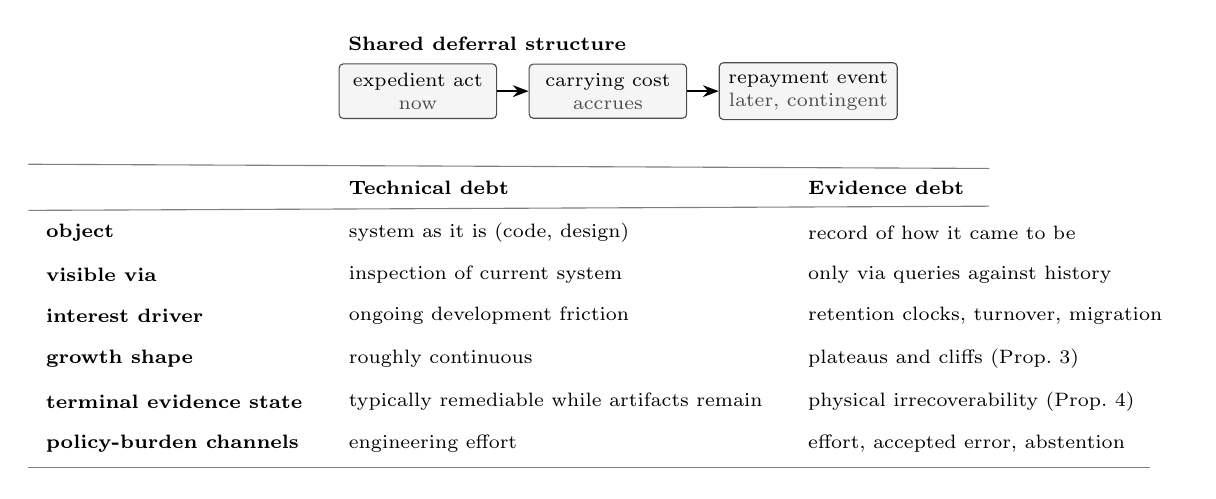
\begin{tikzpicture}[node distance=2.8mm and 4mm]
  % shared structure
  \node[lbl, anchor=west] (h0) at (0,0) {\textbf{Shared deferral structure}};
  \node[stage, below=2.5mm of h0.west, anchor=north west, minimum width=20mm] (a)
    {expedient act\\{\smlbl now}};
  \node[stage, right=4mm of a, minimum width=20mm] (b)
    {carrying cost\\{\smlbl accrues}};
  \node[stage, right=4mm of b, minimum width=20mm] (c)
    {repayment event\\{\smlbl later, contingent}};
  \draw[flow] (a) -- (b);
  \draw[flow] (b) -- (c);

  % divergence table
  \matrix (m) [below=5mm of b, matrix of nodes, column sep=2.5mm, row sep=0.7mm,
    nodes={font=\fontsize{6.8}{7.9}\selectfont, anchor=west, align=left},
    column 1/.style={nodes={font=\fontsize{6.8}{7.9}\selectfont\bfseries}}]
  {
    \strut & \textbf{Technical debt} & \textbf{Evidence debt} \\
    object & system as it is (code, design) & record of how it came to be \\
    visible via & inspection of current system & only via queries against history \\
    interest driver & ongoing development friction & retention clocks, turnover, migration \\
    growth shape & roughly continuous & plateaus and cliffs (Prop.~3) \\
    terminal evidence state & typically remediable while artifacts remain & physical irrecoverability (Prop.~4) \\
    policy-burden channels & engineering effort & effort, accepted error, abstention \\
  };
  \draw[black!50] ($(m-1-1.north west)+(-1mm,0.4mm)$) -- ($(m-1-3.north east)+(1mm,0.4mm)$);
  \draw[black!50] ($(m-1-1.south west)+(-1mm,-0.2mm)$) -- ($(m-1-3.south east)+(1mm,-0.2mm)$);
  \draw[black!50] ($(m-7-1.south west)+(-1mm,-0.6mm)$) -- ($(m-7-3.south east)+(1mm,-0.6mm)$);
\end{tikzpicture}
}
\caption{Technical debt versus evidence debt. Both share the deferral structure
(left): an expedient act now, a carrying cost, a repayment event. They diverge in
every load-bearing property (right): object, visibility, interest driver, growth
shape, terminal state, and repayment currency. The comparison is the condensed form
of \cref{sec:novelty}.}
\label{fig:tdvsed}
\end{figure}

\Cref{fig:tdvsed} condenses the comparison. The claim, precisely bounded: evidence
debt is a member of the debt family by structure, and reducible to no existing
member by object, dynamics, or management levers.

\section{Discussion}
\label{sec:discussion}

\subsection{Attacking the Metaphor, Deliberately}
\label{sec:disc-metaphor}

A concept paper owes its readers the strongest case against itself. We therefore
attack our own framing and report what survives. \emph{Where the financial analogy fails:} there is no
creditor and no contract---nobody agreed to the terms, and the ``lender'' (future
circumstance) never negotiates; effort and abstention exposure under sound exhaustive
policies follow a stochastic
schedule of cliffs and hazards while error may drift with discriminator quality
(\cref{prop:steps}), so compounding
intuitions---and any metric built on them---mislead (\cref{met:interest} was
rejected on exactly this ground); policy burden is not fungible---effort, accepted
error, and abstention (\cref{fnd:effort,fnd:false,fnd:redundancy}) are different
channels that do
not net against each other; and physical irrecoverability boundaries are mandatory and world-imposed
(\cref{prop:writeoff}), where financial write-offs are creditor choices.
\emph{Where the analogy earns its keep:} the deferral structure is real (a present
choice with a later, larger, contingent cost); the principal/carrying-cost
decomposition marks a real operational distinction (capture-time gaps versus
decay-driven growth) with distinct remedies (capture discipline versus retention
and export policy); and ``debt'' correctly imports the management insight that the
stock must be measured and budgeted, not merely deplored.

\emph{The removal test}: delete the word ``debt'' and every construct still
stands---deficit (\cref{def:deficit}) is a syntactic census; reconstruction cost
(\cref{def:rec}) is a measured quantity; decay schedules and half-lives
(\cref{sec:interest}) are computed from published retention and turnover;
irrecoverability (\cref{def:irrec}) is a decidable/certifiable state; and the
expected-excess-burden aggregate (\cref{def:debt}) is an ordinary expected value that
could as well be called \emph{reconstruction exposure}. We embrace that reading:
the \emph{measured} quantity is reconstruction exposure, and a skeptic may use
that vocabulary throughout without loss of formal content.

What, then, does the debt framing add that exposure does not? Exposure language
frames the quantity as environmental---a risk one has, like weather. The debt
framing makes one further, contentful commitment: it binds the aggregate to
\emph{identifiable, dated, attributable deferral decisions}---this change, shipped
ticketless, under this pressure, by this team---and thereby licenses management
machinery that exposure language does not naturally carry: per-decision
registration at creation time (the register of \cref{sec:disc-management}, with
backfill due dates set inside the cheapest-path window); attribution of the
aggregate to controllable practices P1--P8 rather than to fate; and the
inflow/stock separation (\cref{met:growth} versus interest) that tells an
organization whether it is borrowing faster or merely aging. These are decisions
and accountabilities, not measurements; the measurement structure is
metaphor-free, and the metaphor's residual work is to keep the human origin of
the exposure attached to the number. That is a naming choice we defend as
useful---while conceding, per the analysis above, that every quantitative
intuition imported from finance (rates, compounding, refinancing) must be checked
against the model and mostly fails.

Circularity was the other standing risk, and the definitional order of
\cref{sec:definitions} was built against it: deficit is defined without reference
to cost (syntax against a declared schema); cost is defined without reference to
deficit (measured effort of answering queries); debt relates the two through an
explicit counterfactual; and the schema- and workload-relativity are declared
inputs rather than smuggled conclusions. What \emph{is} irreducibly judgmental
---the choice of $\Sch$ and $(w_q, \lambda_q, \pi_q)$---is surfaced as a governance decision,
not hidden in a formula (\cref{sec:model-notformula}).

\subsection{Relativity of the Construct}
\label{sec:disc-relativity}
The sharpest structural limitation is not the metaphor but the relativity:
$\ED$ is defined against a declared schema $\Sch$ and a declared workload
$(w_q, \lambda_q, \pi_q)$, all controlled by the party being measured. An estate can reach
$\ED \approx 0$ by declaring a weak schema or a sparse workload, and
\cref{fnd:ed} showed concretely how the penalty declaration reshapes what the
number says. We therefore state plainly: what is measurable
\emph{inter-subjectively} is the ingredient vector---EDR against a published
schema, measured ERC and FRR under the same stated policy, the decay schedule, and the
irrecoverability constructs---while $\ED$ itself is an accounting quantity
relative to published governance inputs, comparable across estates only under
shared reference declarations and the same $\rho$. Policy choice is another gaming
surface: an aggressive policy can trade $N$ for $W$, while a conservative one does
the reverse. Cross-organizational reporting should therefore publish S/W/N and IRR,
and, where policies differ, report a policy frontier rather than compare scalar
$\ED_\rho$ values as though they shared an estimand. To make comparison possible rather than merely
honest, we propose (as future standardization, not as this paper's result) a
\emph{reference declaration}: the six-interrogative schema of
\cref{sec:schema-informal} as $\Sch_{\mathrm{ref}}$, and a workload
$\Qw_{\mathrm{ref}}$ parameterized by public covariates---per-service audit
queries at a fixed annual rate, incident queries at the estate's measured
incident rate, one recovery query per service---with error and abstention weights published
alongside any reported figure. This is the same discipline financial accounting
imposes through reporting standards: the number is meaningful because the rules
for producing it are shared, not because it is observer-independent.
For initial calibration, teams should derive $w_q$ from observed incident/audit
query counts per reporting horizon or from explicit scenario probabilities;
$\lambda_q$ from the incremental consequence of acting on an accepted wrong answer
(e.g., investigation labor, remediation, or outage minutes); and $\pi_q$ from the
incremental consequence of leaving that same question unresolved. All three must be
expressed in one declared accounting unit. A practical elicitation is to record
low/base/high values with the incident commander, audit owner, and service owner,
then publish both the elicited rationale and the resulting grid. No universal
DORA-derived default exists for these losses; when local estimates are weak, the
honest output is the ingredient vector plus a declared $\lambda/\pi$ grid such as
\cref{tab:pi-sensitivity}, not a falsely precise scalar. IRR remains a separate
physical diagnostic unless a joint loss $L_q(Y_\rho,\mathsf I_q)$ is calibrated.

\subsection{Explanatory and Predictive Value}
The concept must be useful beyond naming. Its explanatory content: it unifies
under one mechanism phenomena currently discussed separately---why incidents on
old systems take longer to diagnose (interest), why audits of healthy systems fail
(deficit despite health), why tool migrations feel like organizational amnesia
(bulk path death), why the departure of one engineer disproportionately damages
some services (human path as last survivor). Its predictive content is concrete
and falsifiable: effort plateaus and cliffs aligned to retention/migration schedules (IH1),
departure-boundary cost multiples (IH2), memory as modal final path (IH3), and
the simulation-grounded expectation that effort inflation precedes failure
(\cref{fnd:effort}). Accepted wrong answers occur, but the isolated density trend
is mixed (\cref{fnd:false}). \Cref{sec:field} specifies the refutation
conditions; a concept that survives them will have earned its place, and one that
does not will have been usefully eliminated.

\subsection{Management Implications (Proposals)}
\label{sec:disc-management}
Stated as proposals, not findings. \emph{Evidence-debt register}: like a TD
register~\cite{seaman2011,ernst2015}, an explicit ledger of known deficits with
principal estimates and decay deadlines---P2 break-glass changes, for instance,
entered at creation with a backfill due date inside the cheapest-path window
(\cref{sec:interest-worked}). \emph{Retention as governance, not default}:
\cref{sec:interest-halflife}'s observation that half-lives are set by unexamined
vendor defaults makes retention review the highest-leverage, lowest-cost
intervention. \emph{Backfill sprints as repayment}: deliberate reconstruction of
high-value history while paths are cheap---though \cref{fnd:false} warns that late
backfill in dense estates risks writing confident fiction into the record, so
backfilled facts should carry confidence annotations. \emph{Deferral budgets}:
if evidence capture is to be skipped under pressure, the skip should be a recorded
decision---the debt family's central lesson~\cite{kruchten2012} transposed: unmanaged
debt is not the debt you took on but the debt you never knew you took on.
\emph{Capture-versus-risk gate}: for capture action $a$ over horizon $H$, record
\[
K_H(a)=K_{\mathrm{labor}}(a)+K_{\mathrm{storage}}(a)
       +K_{\mathrm{privacy/control}}(a),
\]
and adopt $a$ when
\[
K_H(a)<\sum_s p_s\bigl[\ED_{\rho,s}^{\neg a}
                         -\ED_{\rho,s}^{a}\bigr],
\]
with scenario probabilities, horizon, accounting unit, and uncertainty range
published. Otherwise selective omission may be rational.
The comparison must be recorded because high-volume controllers can make exhaustive
capture technically or legally disproportionate. This is a decision rule proposal,
not a claim that this paper has measured either side of the trade-off; it closes the
decision logic without pretending that the synthetic study supplies capture costs.

\subsection{Limitations}
Beyond the simulation threats (\cref{sec:sim-threats}): the framework prices
reconstruction, not the first-order value of evidence for real-time operations
(alerting, debugging), which observability already treats~\cite{majors2022}; the
workload $\Qw$ is a declared judgment and organizations may declare it
self-servingly---the discipline is publishing it; capture itself has costs
(effort, storage, privacy exposure under data-protection law~\cite{gdpr,
nist80092}) that our gate parameterizes but this study does not calibrate, so the
empirical optimization of capture under cost and legal constraint remains open;
and the only non-synthetic observation is a bounded, age-stratified public-forge
sample that shows missing external issue linkage occurs under a declared schema
but measures neither intent adequacy, decay, reconstruction, nor money
(\cref{tab:argocd-census}). All cost, error, interaction, and debt magnitudes remain
synthetic, a boundary marked at every claim.

\section{Conclusion}
\label{sec:conclusion}

Cloud-native operations have made change cheap, fast, and voluminous---and have
thereby made the \emph{record} of change the system's most perishable component.
This paper named the resulting deferred cost evidence debt and did the work the
name requires: non-circular definitions grounded in observables; a formal model in
which debt is expected excess reconstruction cost, reconstruction is linkage
inference, and decay is a survival process; analytic results locating exactly where
the financial metaphor breaks (stochastic step interest, mandatory write-offs) and
what remains when it is removed; a metric suite honest enough to reject one of its
own commissioned members; an executed, fully reproducible degradation experiment
showing that redundancy absorbs small deficits, that deficit classes collapse
reconstruction superadditively, that effort inflates before failure appears, and
that reconstruction under heavy deficit fabricates confident false history at rates
that should alarm anyone who has trusted an after-the-fact timeline; a bounded,
age-stratified Argo CD observation showing that missing external issue linkage
occurs in public repository evidence while review-record and release-lineage
presence controls remain high; and a field protocol with stated refutation
conditions. The repository observation is not a measurement of intent quality,
decay, evidence debt, or reconstruction cost.

The central claim---deferral without elimination---emerges from this treatment
with its proper status: not an axiom but a structured hypothesis, true in the
simulation's closed world in a specific, mechanistic way (payment in effort, then
error, then loss), and awaiting field magnitudes. The constructs are offered for
reuse: a deficit census any organization can run, a decay schedule any organization
can read off its own retention settings, and a definition of debt that makes the
implicit question---\emph{what will it cost us to not know what we did?}---explicit,
estimable, and budgetable. Systems will keep forgetting; the choice organizations
retain is whether the forgetting is priced.


\balance
\bibliographystyle{ieeetr}
\bibliography{refs}

\end{document}
